\addtocontents{toc}{\protect\newpage}
\chapter{Evaluation}
\label{sec:eval}

This chapter investigates the performance of presented approaches and variants to EV scheduling in relation to the pre-defined reference cases, summarised in \Autoref{tab:casestuds}. In \Autoref{sec:ec} the characteristics of the reference optimisations are reiterated, and evaluation criteria whereby effectiveness will be assessed are introduced. \Autoref{sec:hmlp} compares the performance of different configurations of network-constrained heuristics and linear programming before uncertainty mitigation options are applied in \Autoref{sec:saunc}. Parametrisation options are, first, interpreted individually and then applied conjointly in \Autoref{sec:joint}. While the preceding sections judge based on the aggregate of 20 scenarios corresponding to a four week weekday period to hedge against the variability of performances across different situations, \Autoref{sec:sceneval} picks a single scenario for an in-depth analysis. \Autoref{sec:hdeval} provides insight into peculiarities on an individual household level before results are discussed, and potential is analysed in \Autoref{sec:pseval}. This is associated with a sensitivity analysis of market price spreading factors towards cost savings.

\begin{table}[]
	\centering
	\scriptsize
	\begin{tabular}{@{}lllll@{}}
		\toprule
		\textbf{Case Studies}  & \textbf{Variants}        &                         &                       &                             \\ \midrule
		Reference Cases        & No Electric Vehicles     & Uncontrolled Charging   & Price-Based Heuristic &                             \\ \midrule
		Heuristics             & Availability             & Battery SOC             & Distance (asc.)       & Distance (desc.)            \\ \midrule
		Linear Programming     & Unconstrained Modulation & Constrainted Modulation & Combined Mitigation   &                             \\ \midrule
		Uncertainty Mitigation & \textit{Availability}    & \textit{Battery SOC}    & \textit{Market Price} & \textit{Res. Demand} \\  \cmidrule{2-5}
		& $\nu_\alpha = 0.6$       & $\nu_B = 0.6$           & $\nu_\pi = 0.90$      & $w = 0.5 $ h                 \\
		& $\nu_\alpha = 0.7$       & $\nu_B = 0.7$           & $\nu_\pi = 0.95$      &                             \\
		& $\nu_\alpha = 0.8$       & $\nu_B = 0.8$           & $\nu_\pi = 0.99$      &                             \\ \bottomrule
	\end{tabular}
	\caption{Summary of evaluated case studies}
	\label{tab:casestuds}
\end{table}

\section{Evaluation Criteria and Reference Cases}
\label{sec:ec}

To facilitate a concise comparison between the scheduling approaches, boxplots are used to indicate the distributions (illustrated by quartiles and whiskers) and averages (denoted by circles) of evaluation criteria throughout the 20 scenarios. Particularly concerning costs, the results are set in relation to the results of uncontrolled charging and the purely price-based heuristic. Recall that three major areas of concern determine the performance of a scheduling approach: cost savings from devised charging, a full battery at the end of the charging period, and the observation of network constraints. These lead to the following evaluation criteria which are inspected separately as no trade-offs are quantified.

\begin{itemize}
	\item \textbf{Relative charging costs} offer insight into the economic benefit of coordinated charging compared to uncontrolled charging as well as a proxy for the costs of introducing network constraints if compared to unconstrained price-based charging.
	\item \textbf{Demand satisfaction} is measured by both the average and minimum final battery state of charge of the controlled vehicles. The latter gives an indication of an algorithm's reliability to provide a minimum driving range to the customer.
	\item \textbf{Severity of constraint violations} is quantified by maximum line loadings and the minimum bus voltages occurring at the households throughout the optimisation horizon.
	\item \textbf{Frequency of constraint violations} is measured by relating the number of overloads or voltage violations to the total number of values measured.
\end{itemize}

\begin{figure}[]
	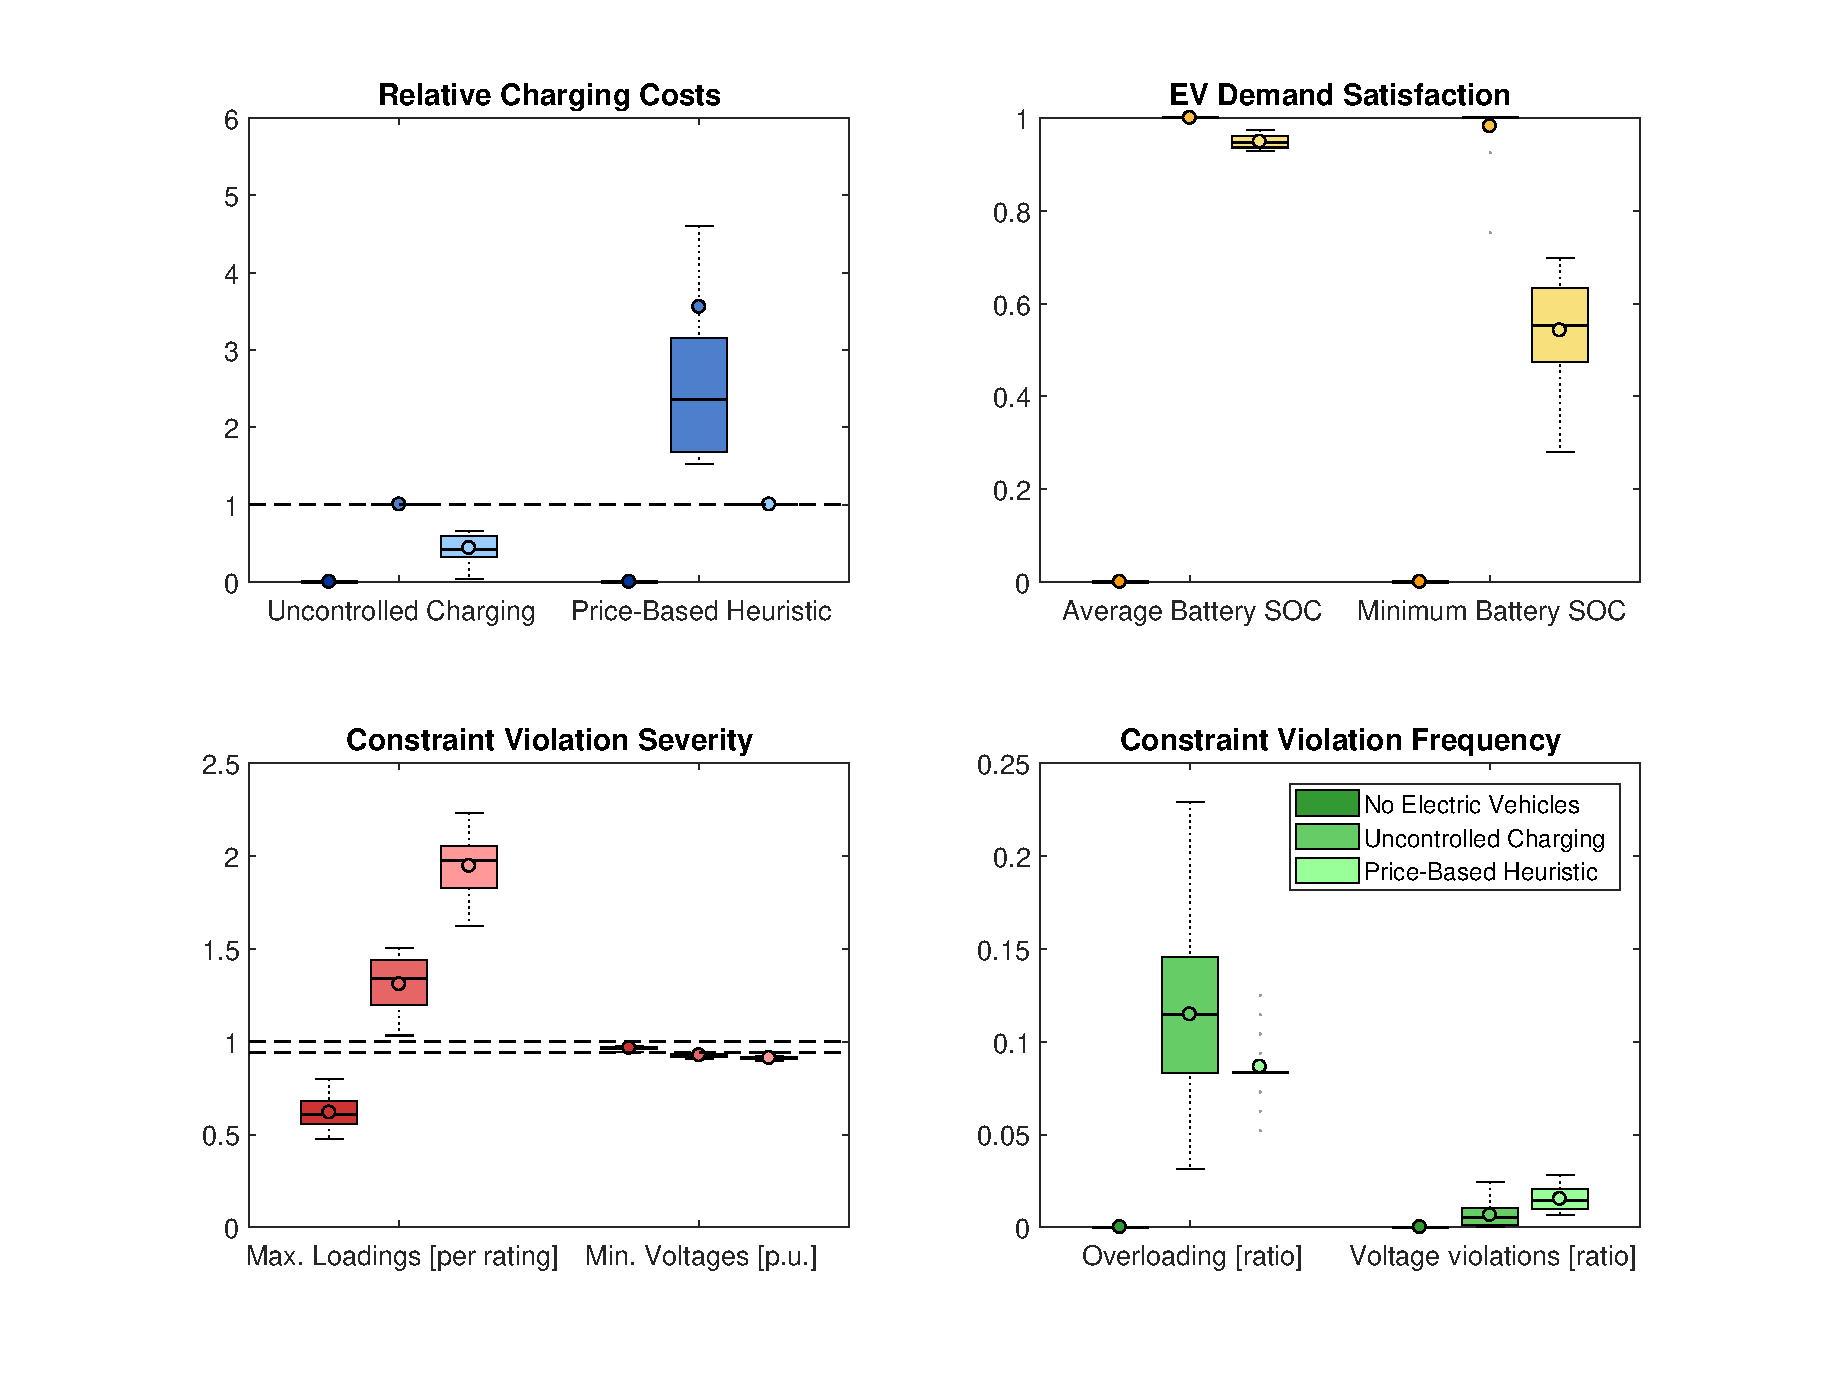
\includegraphics[width=\textwidth,trim={3cm 1.5cm 2.5cm 0cm},clip]{figures/evaluation/refcases.eps}
	\caption{Benchmark of reference cases: no EVs, uncontrolled charging, and price-based heuristic}
	\label{fig:refcases}
\end{figure}

Initially, a look at the performance of the benchmarks in \Autoref{fig:refcases} affirms their unsuitability to achieve safe, reliable, and cheap EV charging. While the price-based heuristic excels at reducing charging costs to about one half compared to uncontrolled charging, it fails to guarantee a full battery state of charge which is due to the day-ahead scheduling involving uncertain parameters. Conversely, the uncontrolled charging stands out with its advantage of operating in real-time and can almost guarantee a full battery. Still, the possibility exists that charging cannot be completed for the EV availability is too limited. Despite the shortcomings of day-ahead scheduling, an average fulfilment ratio of vehicle demand of 94.86\% is considerable and covers most daily trip lengths. However, due to reliability concerns the minimum battery SOC is the more critical performance measure influencing customer acceptance, which averages at only 54.17\%.

\newpage
A glance at the maximum line loadings and minimum voltages reveals that without electric vehicles the test network is perfectly healthy; no violations occur. Yet, the presence of uncontrolled EV charging causes voltage violations and overloads in any scenario averaging at an excess loading of 30.84\%. Due to the natural spread of arrival times, the overloads are nowhere near the overloads caused by applying the price-based heuristic averaging at a 94.63\% excess loading. Analogous findings could be made for minimum bus voltages. The fact that charging concentrates in the single cheapest slots coupled with high availability rates reiterates the need for charging coordination of electric vehicles if general price-based incentives are given.

In terms of violation frequency, the price-based heuristic also entails more voltage issues than uncontrolled charging because the high peak loads -- in addition to the increased likelihood \textit{that} a voltage violation occurs -- not only deteriorates voltages locally but will also propagate along the feeder. Because of the peakiness of the schedule overloads of the mains cable are less frequent than invoked by uncontrolled charging, again due to the natural arrival time spread. While loads still occur in periods of peak residential demand, they distributed over that period such that line limits are continuously exceeded.

\section{Performance of Heuristic Modes and Linear Programming}
\label{sec:hmlp}

Having analysed the reference cases, the different network-constrained heuristic modes were run as outlined in the introduction to this chapter, with priority lists determined by the rank of availability period, initial SOC, ascending or descending distance from the substation. \Autoref{fig:heulp} summarises the performance of applied charging schemes. Relatively similar charging costs are achieved regardless of the priority list used by which EVs are scheduled. All were able to reduce costs by approximately 54\% compared to uncontrolled charging for the given market assumptions (spreading factor $s=5$), the sensitivities to which are addressed later in \Autoref{sec:pseval}. Noteworthily, other than expected the ordering by ascending distance does not improve costs, and no financial benefit could be drawn from maximum capacity exploitation in cheap slots. Instead, prioritising by initial SOC convinces with a slight advantage of 1\% with respect to cost increase due to technical constraints. The lower deviation of the price-based heuristic costs by the network-constrained variants is obtained through favourable price forecast variations in slots where the latter charges more than the former and this would not be possible if no uncertainty were involved. While the average fulfilment ratio of EV demands remains indistinguishable at 94.80\% across different heuristic configurations, the minimum reached battery charge level of vehicles under the aggregator's control is minimally less for mode `SOC' and `descending distance'.

Concerning the technical performance of the heuristic modes, it can be noticed that the marginal economic advantage of mode `SOC' is paid with an increased risk of overloading of the mains cable and local voltage violations. Although in the vast majority of cases network constraints are observed, they are not precluded. Importantly, other than for the uncoordinated reference cases, overloads induced by the network-constrained heuristics are limited to marginal overloads of up to 2\% which are most likely due to an unfavourable shift in residential loads. The linear power flow approximation continued to yield overestimates and did not contribute to these overloads.

\begin{figure}[]
	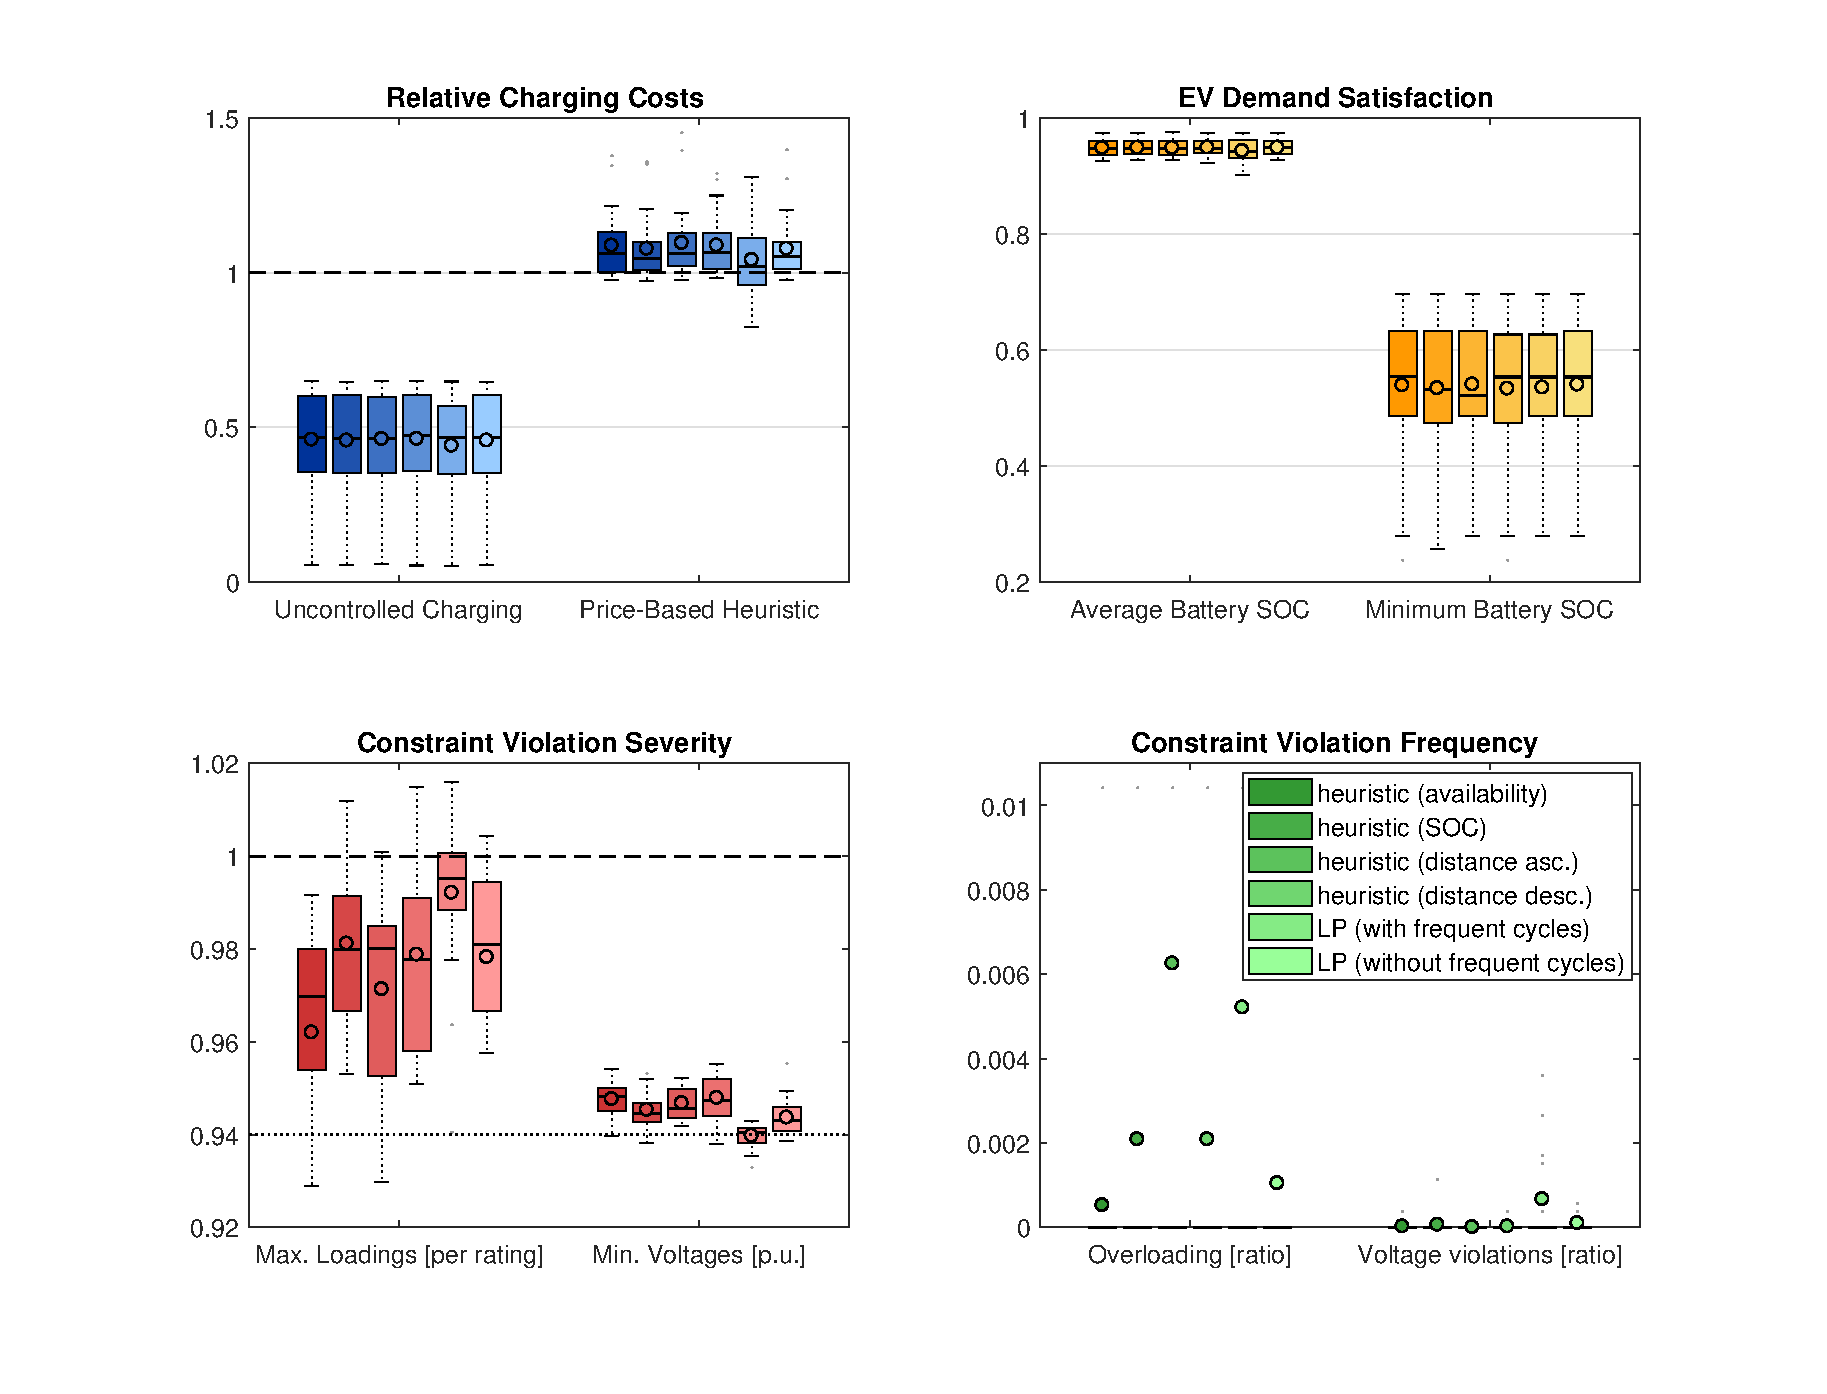
\includegraphics[width=\textwidth,trim={2.9cm 1.5cm 2.5cm 0cm},clip]{figures/evaluation/heulp.eps}
	\caption{Performance of heuristic optimisation modes and linear programming}
	\label{fig:heulp}
\end{figure}

The linear programme (LP) was run in two variants. First, with unconstrained charge rate modulation allowing frequent on/off cycles and, second, with constrained charge rate modulation as prescribed in the constraint formulated in \Autoref{eq:crm} which could not be recognised in heuristic scheduling. The LP allowing frequent cycling achieves another 1.6\% cost reduction compared to uncontrolled charging averaging at 43.99\%, whereas virtually no change in relative charging costs could be observed for the LP including the charge rate modulation constraint. 

However, because the latter obstructs maximum charging rates on the edges of the availability period, but requires slow ramping of charging rates, the average fulfilment ratio of demand stabilises on the niveau of the heuristics, which had deteriorated marginally for the unconstrained LP. Likewise, in the technical domain, the LP with restricted charge rate modulation outperforms its unconstrained pendant. More than half of the analysed scenarios exhibits some voltage violations in the network, whereas this is reduced to a fraction for the constrained LP.

In general, the fact that the cost increase from unconstrained to network-constrained optimisation is confined to the order of 10\% on average is remarkable. Since it was established that the price-based heuristic causes severe slot-wise violations, this indicates that numerous alternative slots with similar charging costs and suitable capacities are available limiting the financial impact of network constraints.

\section{Sensitivity Analysis of Uncertainty Mitigation Approaches}
\label{sec:saunc}

This section analyses the sensitivity of algorithm performance to different parameter configurations of the uncertainty mitigation approaches presented in \Autoref{sec:uncmitigation}. The parameters mirror varying degrees of conservatism and determine the extent of security margins applied. The base case for comparison was chosen to be the LP with constrained charge rate modulation.

\subsection{Vehicle Availability Uncertainty Attenuation}

\Autoref{fig:lpav} reveals a limited effect for availability uncertainty attenuation in non-technical regards: except for a minor improvement in minimum battery charge levels from 54.00\% to 54.83\% on average at negligible extra cost, no refinement could be noted. A reason for the limited effect of availability uncertainty mitigation falling short of expectations is that the slow ramping of charging rates in the LP already mitigates inherently by not allocating maximum charge rates in rather uncertain boundary regions of predicted availability. Nonetheless, this approach constitutes a valuable addition if a charge rate modulation constraint is not imposed. %PROOF!

\begin{figure}[]
	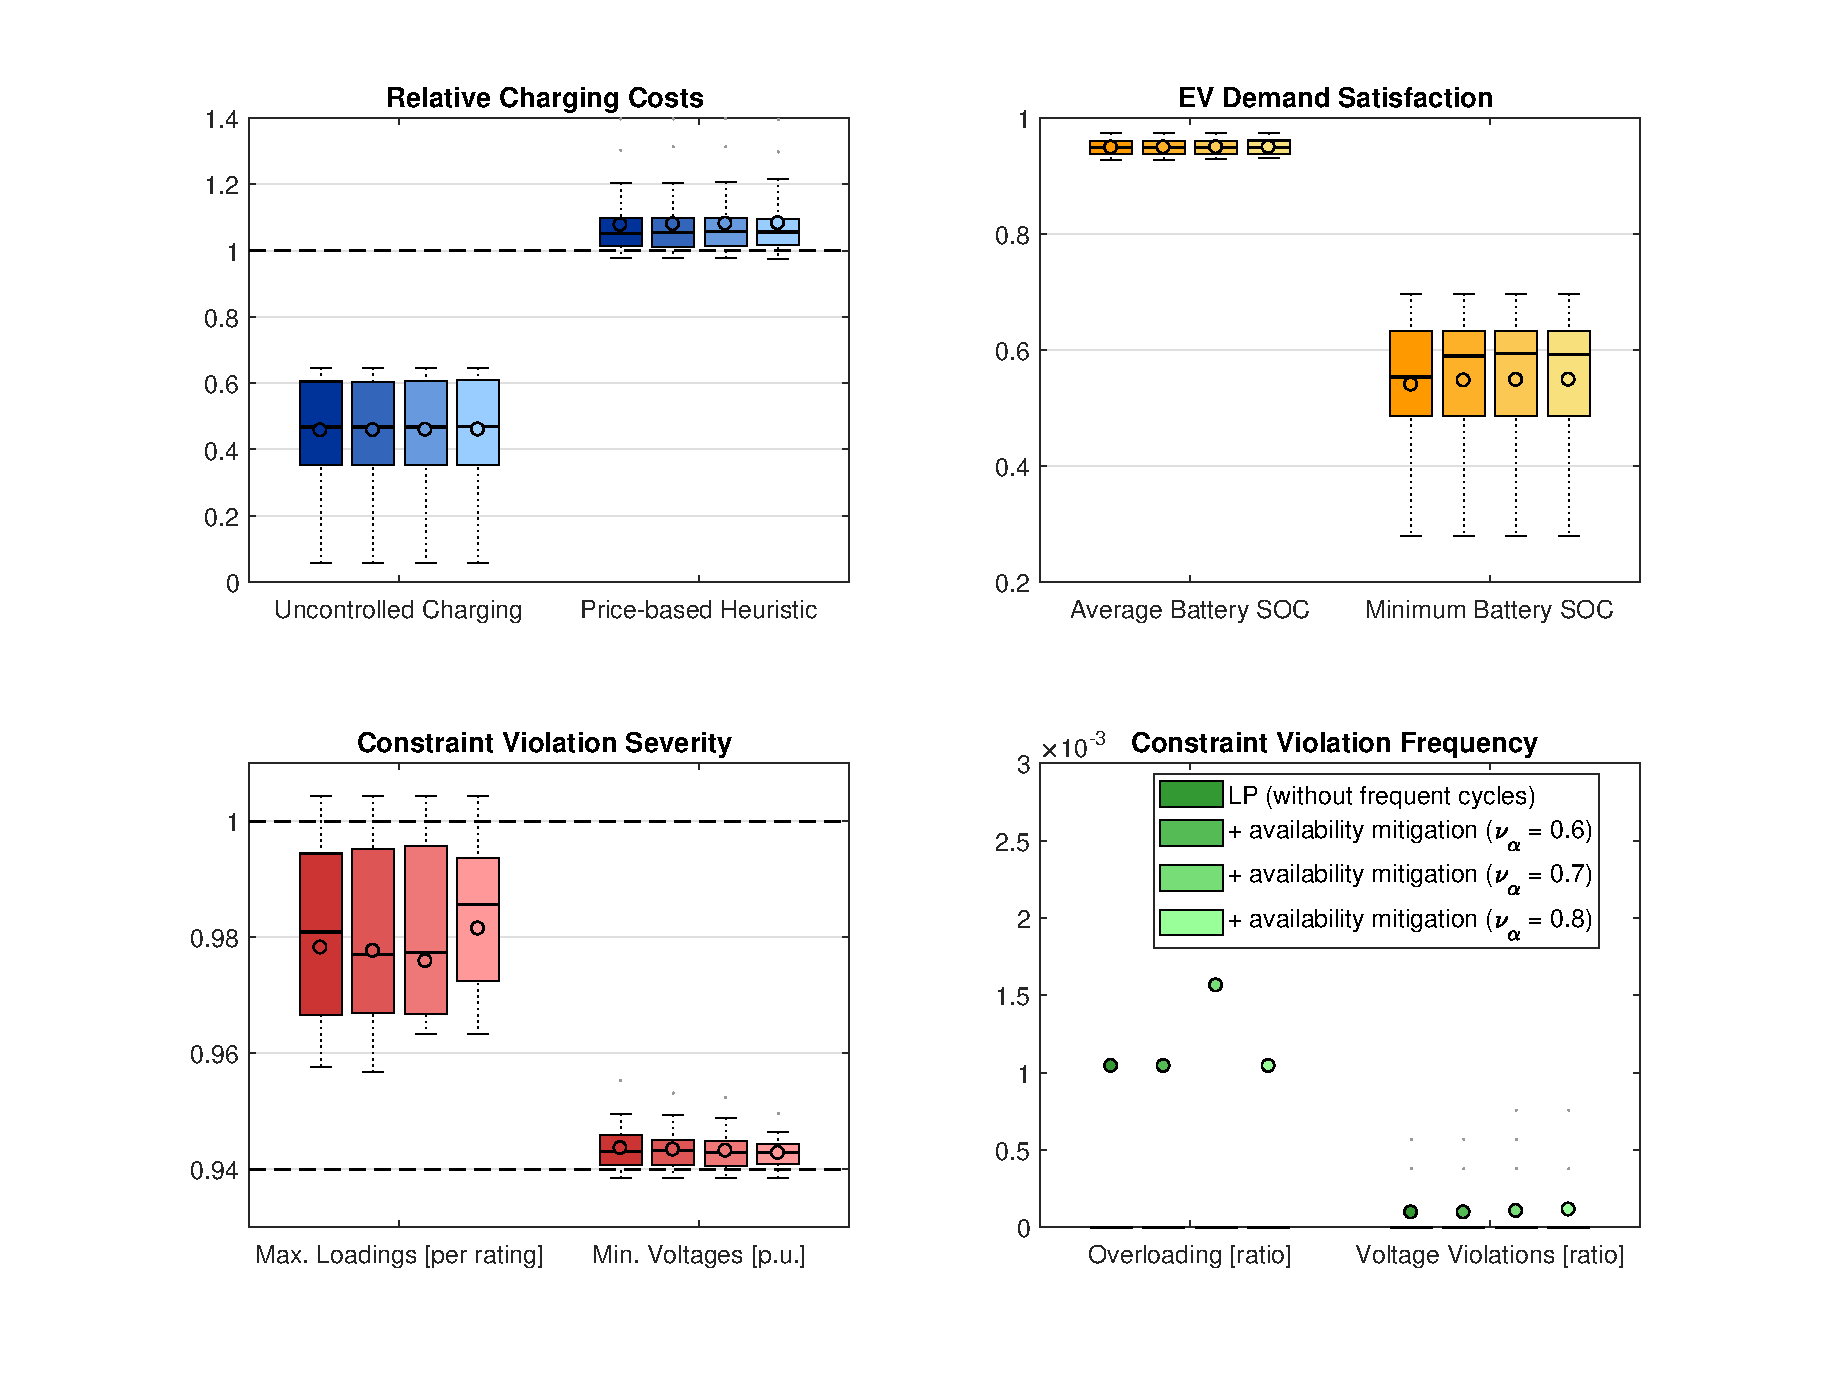
\includegraphics[width=\textwidth,trim={2.9cm 1.5cm 2.5cm 0cm},clip]{figures/evaluation/lp_av.eps}
	\caption{Sensitivities of availability uncertainty mitigation parameters}
	\label{fig:lpav}
\end{figure}

Technically, discernible changes are observed exclusively for high security margins. The average line loading increases, while voltages tend to deteriorate marginally. This effect is induced by the limited load flexibility of electric vehicles due to a high level of conservatism and, thus, constellations in which loads aggregate on fewer slots even if sub-optimal. By subjective weighting, parameter $\nu_{\alpha}=0.6$ is chosen to enter into the joint mitigation parameter set.

\subsection{Battery State of Charge Uncertainty Attenuation}

Battery state of charge uncertainty mitigation summarised in \Autoref{fig:lpsoc} yields results as intuitively expected. With increasing security constraints, while charging costs increase, the reliability of EV demand satisfaction rises; especially the minimum final battery charge increases rapidly. Charging for a battery state of charge that is not lower in 80\% of all cases leads to satisfaction rates of more than 98.18\% on average compared to previously 94.86\% and minimum charge levels of 74.08\% rather than mere 54.00\% for a limited increase in costs of 10\%. Because electric vehicles are scheduled to provide more energy than they are actually expected to require, necessarily some schedule slots will remain unused and may not coincide with the most economical benign slots if simply cut off by a controller once a full charge is reached.

\begin{figure}[]
	\centering
	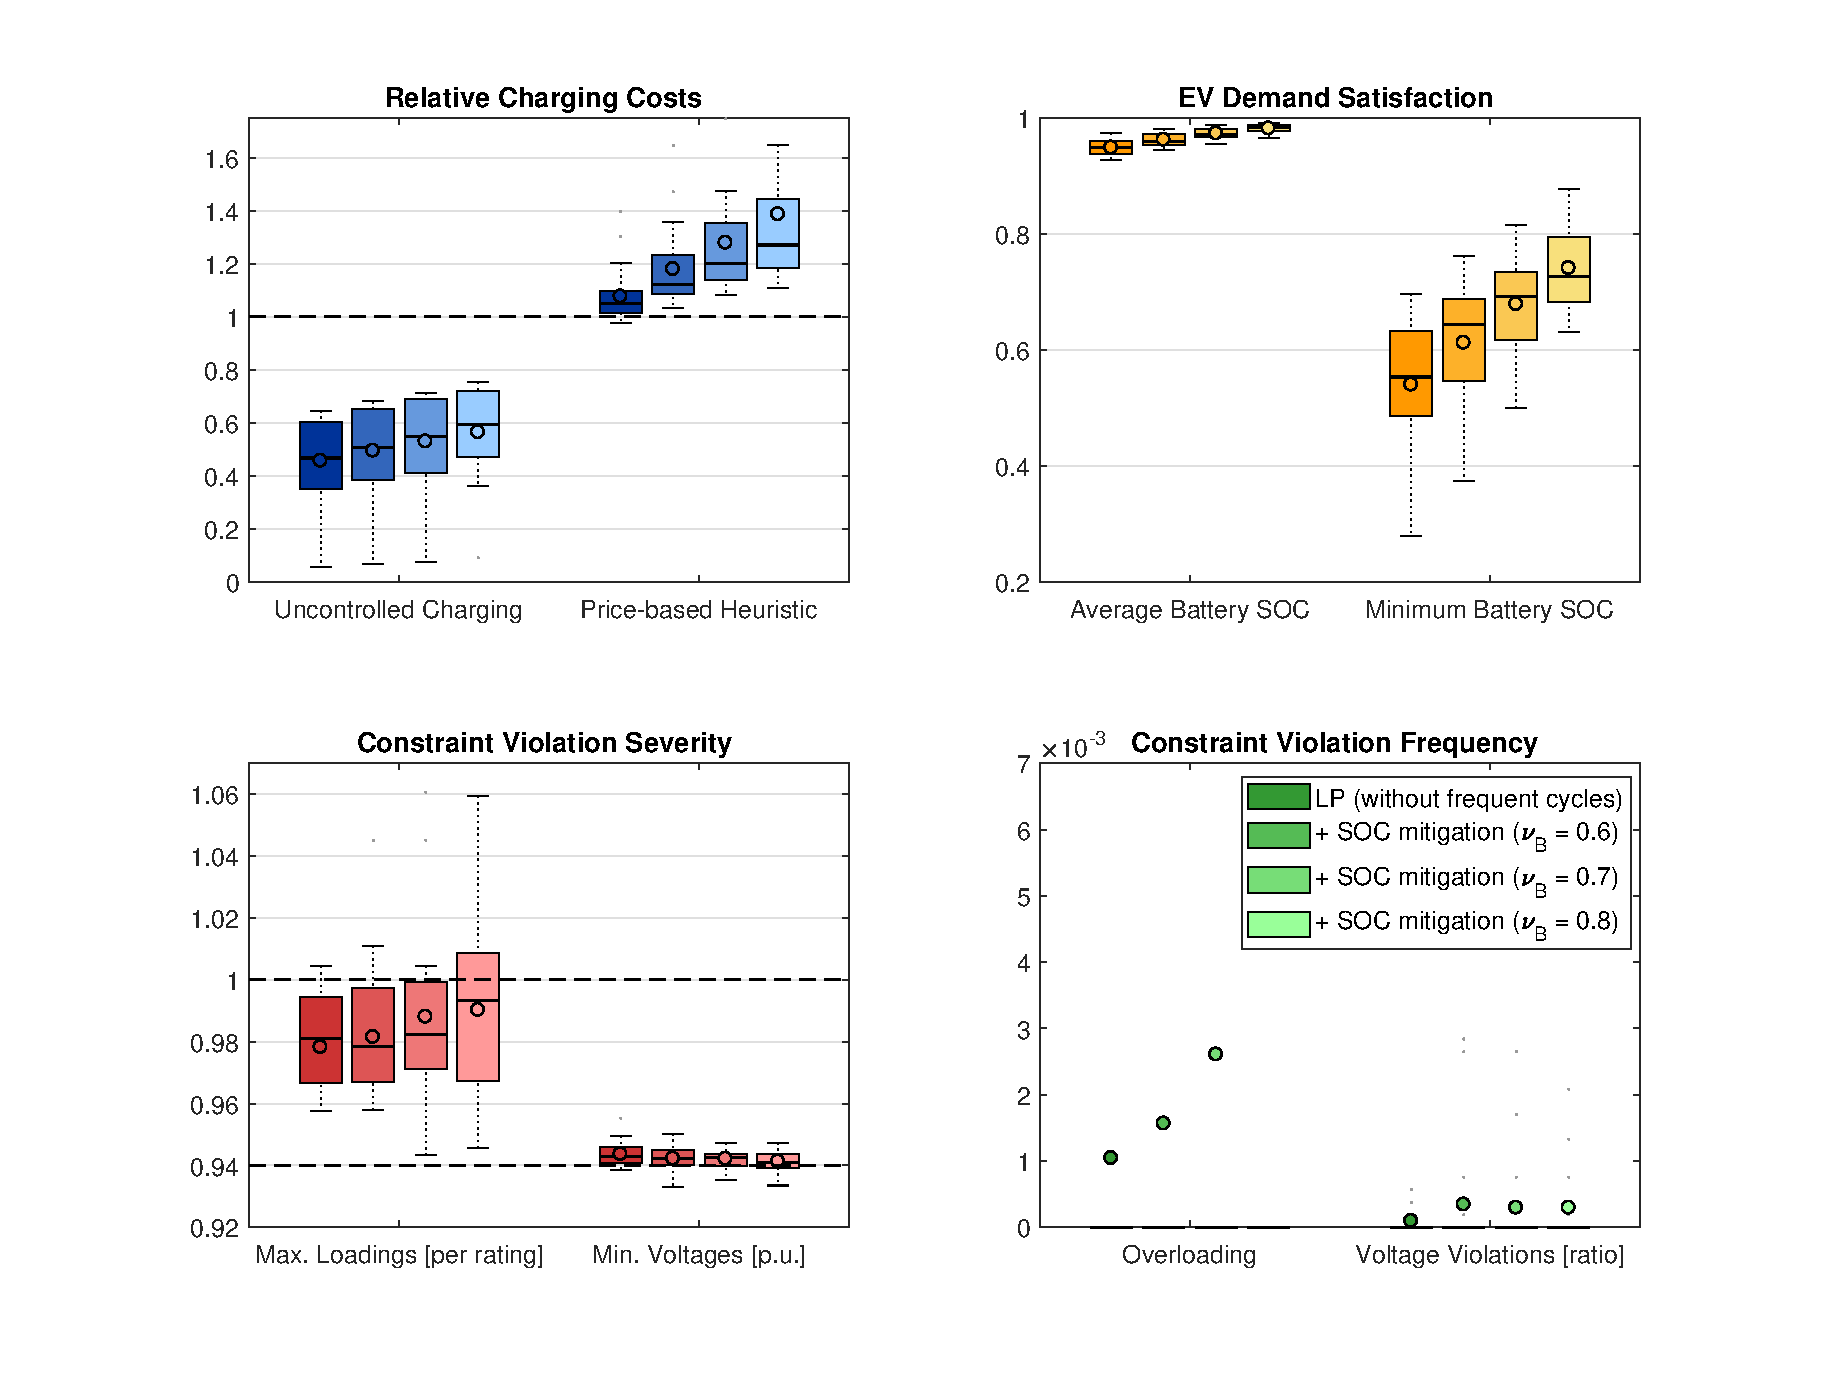
\includegraphics[width=.98\textwidth,trim={2.9cm 1.7cm 2.5cm 0.9cm},clip]{figures/evaluation/lp_soc.eps}
	\caption{Sensitivities of daily mileage uncertainty mitigation parameters}
	\label{fig:lpsoc}
\end{figure}

\newpage
A more intelligent controller might alleviate this price rise by deleting the most expensive redundant slots from the schedule after arrival and knowledge about the battery state of charge is available. Nonetheless, with either type of controller charging will be more expensive as there is a trade-off between granting an electric vehicle flexibility and blocking cheap time slots for others. The unused scheduled charge rates of one electric vehicle could have potentially reduced costs for another and freed network capacity in inexpensive slots stays unexploited. Therefore, the increased satisfaction levels of EVs participating in controlled charging is purchased by a suboptimal allocation of finally realised charging processes.

Moreover, the flexibility through this form of uncertainty mitigation fosters the violation of network constraints as loads must partially be allocated in slots where inhabitants are active, and residential electricity demand is inflicted with more substantial uncertainties. Again, the parameter $\nu_{B}=0.7$ is subjectively chosen for the joint mitigation parameter set. Higher security margins were excluded as these yielded frequent infeasible problem formulations as too much load was demand under given constraints.

\subsection{Market Price Uncertainty Attenuation}

The application of market price uncertainty mitigation is effective at reducing the uncertainty about realised charging costs. \Autoref{fig:lppr} illustrates how the range of deviations of simulated charging costs from the predicted costs of the schedule shrinks with increasing security margins $\nu_{\pi}$. Particularly the step from $\nu_\pi=0.95$ to $\nu_\pi=0.99$ is very effective, which is underlined by the compilation of ranges in \Autoref{tab:costrange}. As this is achieved by shifting the schedules away from the most inexpensive but highly uncertain slots, an average cost increase of 2.34\% from \pounds 44.32 to \pounds 45.35 results. Because of the little distortion of price ranking, for lower $\nu_{\pi}$ the approach is ineffective. In conclusion, efficacy requires alterations in the price ranking.

\begin{figure}[]
	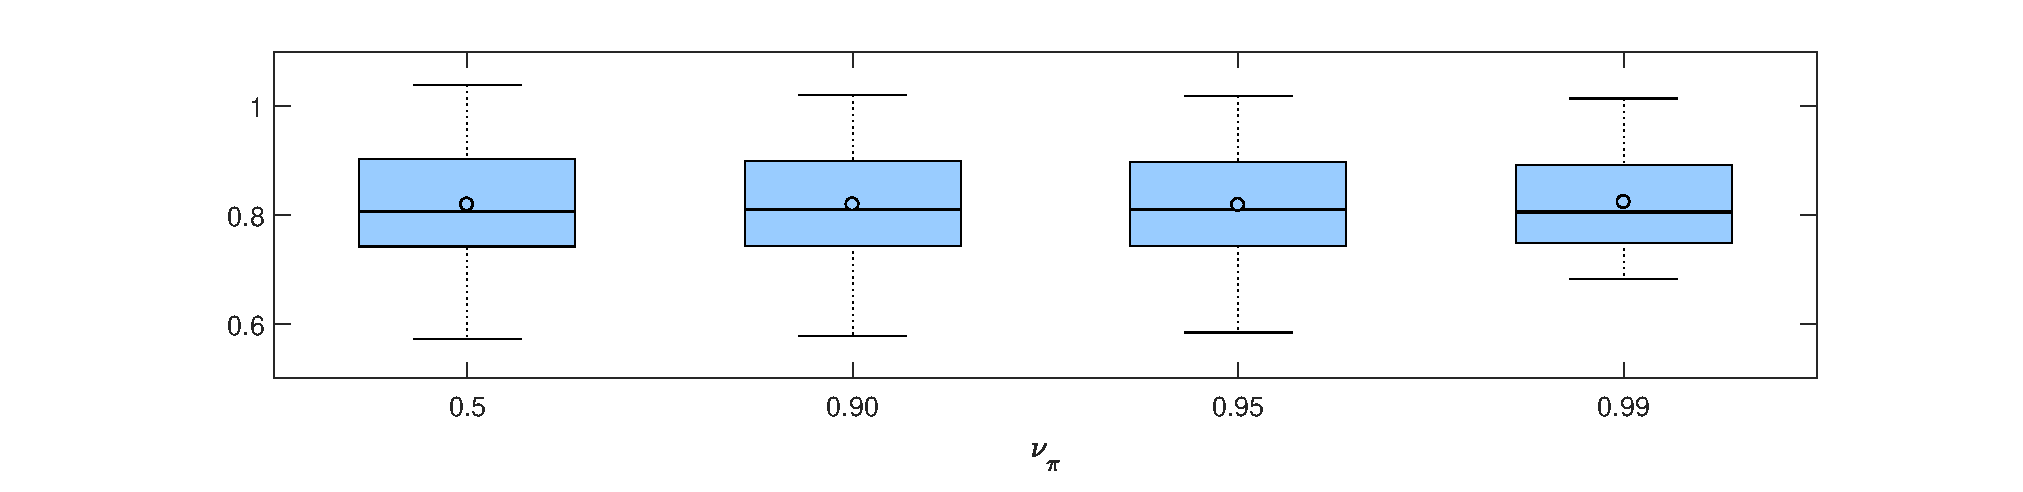
\includegraphics[width=\textwidth,trim={2.9cm 0cm 2.5cm 0cm},clip]{figures/evaluation/lp_pr2.eps}
	\caption[Sensitivity of price uncertainty mitigation parameters]{Simulated costs in relation to predicted costs of schedule with varying price uncertainty mitigation parameters. Shows the sensitivity of price uncertainty mitigation.}
	\label{fig:lppr}
\end{figure}

\begin{table}[]
	\centering
		\begin{tabular}{@{}llllll@{}}
			\toprule
			$\nu_\pi$ & \textbf{0.5}   & \textbf{0.90}   & \textbf{0.95}   & \textbf{0.99}  & \textbf{[unit]} \\ \midrule
			Maximum & 1.039 & 1.020 & 1.019 & 1.014 & - \\
			Minimum & 0.573 & 0.578 & 0.884 & 0.683 & -\\
			Range     & 0.466 & 0.442 & 0.434 & 0.331 &-  \\
			Average simulated costs & 44.32 & 44.43 & 44.43 & 45.35 & \pounds\\ \bottomrule
		\end{tabular}%
	\caption[Sensitivity of price uncertainty mitigation parameters]{Ranges of simulated costs in relation to predicted costs of schedule with varying price uncertainty mitigation parameters. Shows the sensitivity of price uncertainty mitigation.}
	\label{tab:costrange}
\end{table}

\subsection{Residential Demand Uncertainty Attenuation}

With little to no infringement on charging costs or satisfaction of electric vehicle demand, the introduction of a demand mitigation approach with a rolling maximum demand profile recognising a 30-minute window size for residential loads entailed a substantial improvement of the schedules' technical performance as depicted in \Autoref{fig:lpdem}. Both overloads and voltage violations were eliminated in all sampled scenarios. Hence, it constitutes a valuable addition to the EV scheduling approach and will be reflected in the joint mitigation with $w = 0.5$h. Similar to the battery uncertainty mitigation, no larger windows were regarded as these would engender intrinsic overloads and voltage violations even without the presence of EVs and grant no possibility to accommodate EV loads in remaining network capacity.

\begin{figure}[]
	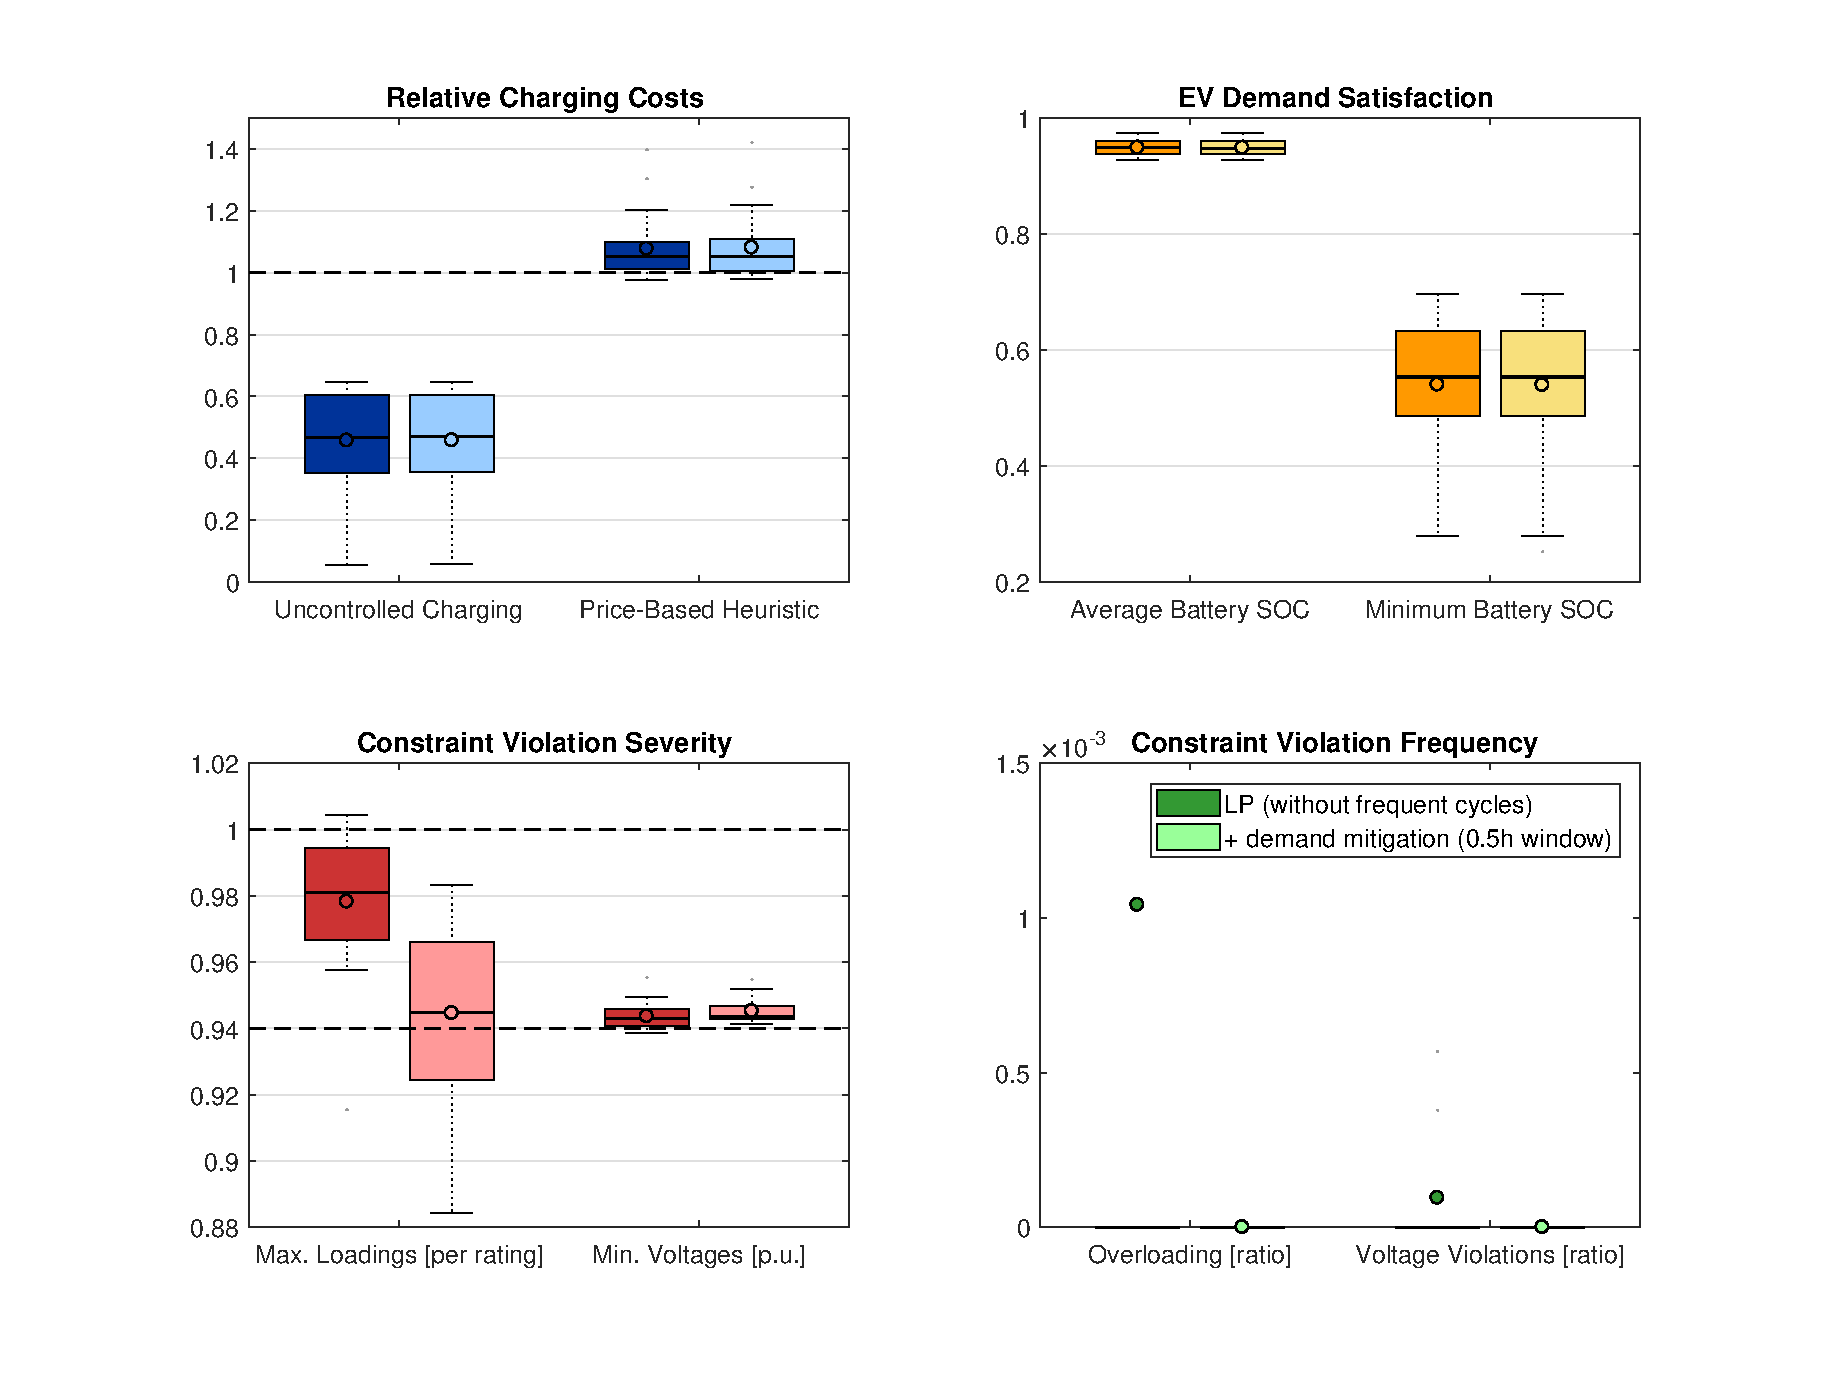
\includegraphics[width=.98\textwidth,trim={2.9cm 1.7cm 2.5cm 0.9cm},clip]{figures/evaluation/lp_dem.eps}
	\caption{Sensitivities of demand uncertainty mitigation parameters}
	\label{fig:lpdem}
\end{figure}

\subsection{Joint Uncertainty Attenuation}
\label{sec:joint}

Individual uncertainty mitigation options have shown that benefits can be drawn to varying degrees. Recall that adapting demand and battery charge level parameters have shown most improvements. It is, however, also vital to evaluate the EV scheduling optimisation, when multiple mitigation approaches are applied simultaneously. As previously noted, too extreme degrees of conservatism may obstruct the feasibility of the problem formulation. Jointly applying security margins to multiple uncertain input parameters bear the potential to be prohibitive and, therefore, are put in a broader perspective via a comparison to the best heuristic and the two LP variants as summarised in \Autoref{fig:joint}.

Indeed, the joint uncertainty mitigation serves its purposes and is generally feasible for the selected subset of parameters. First, the fulfilment ratio of both minimum and average demand could be enhanced to 68.57\% and 97.37\% respectively. Second, neither do voltage violations occur nor are thermal line ratings exceeded. Whether the advantage in EV demand satisfaction on the customer side and the observation of network constraints on the distribution system operator side are worth the reduced cost savings in the order of 10\% in comparison to uncontrolled charging could be based on a willingness to pay or, more accurately, get paid approach. By surveying EV owners the value of a conceivable compensation paid by the aggregator for not completely charging the corresponding battery is determined. Likewise, the inclination of the distribution network operator to appreciate the robustness of the adapted EV schedules depends on the DNO's toolbox, i.e.\ what are its alternative means to overcome unplanned voltage drops or excess demand in the network and what are their respective operating cost. Both considerations are pivotal for the real implementation of the scheduling method but require rigorous analysis of another domain. Instead, this work focusses on what the cost is and eludes a recommendation whether the increase in costs is economically justified.

\begin{figure}[]
	\centering
	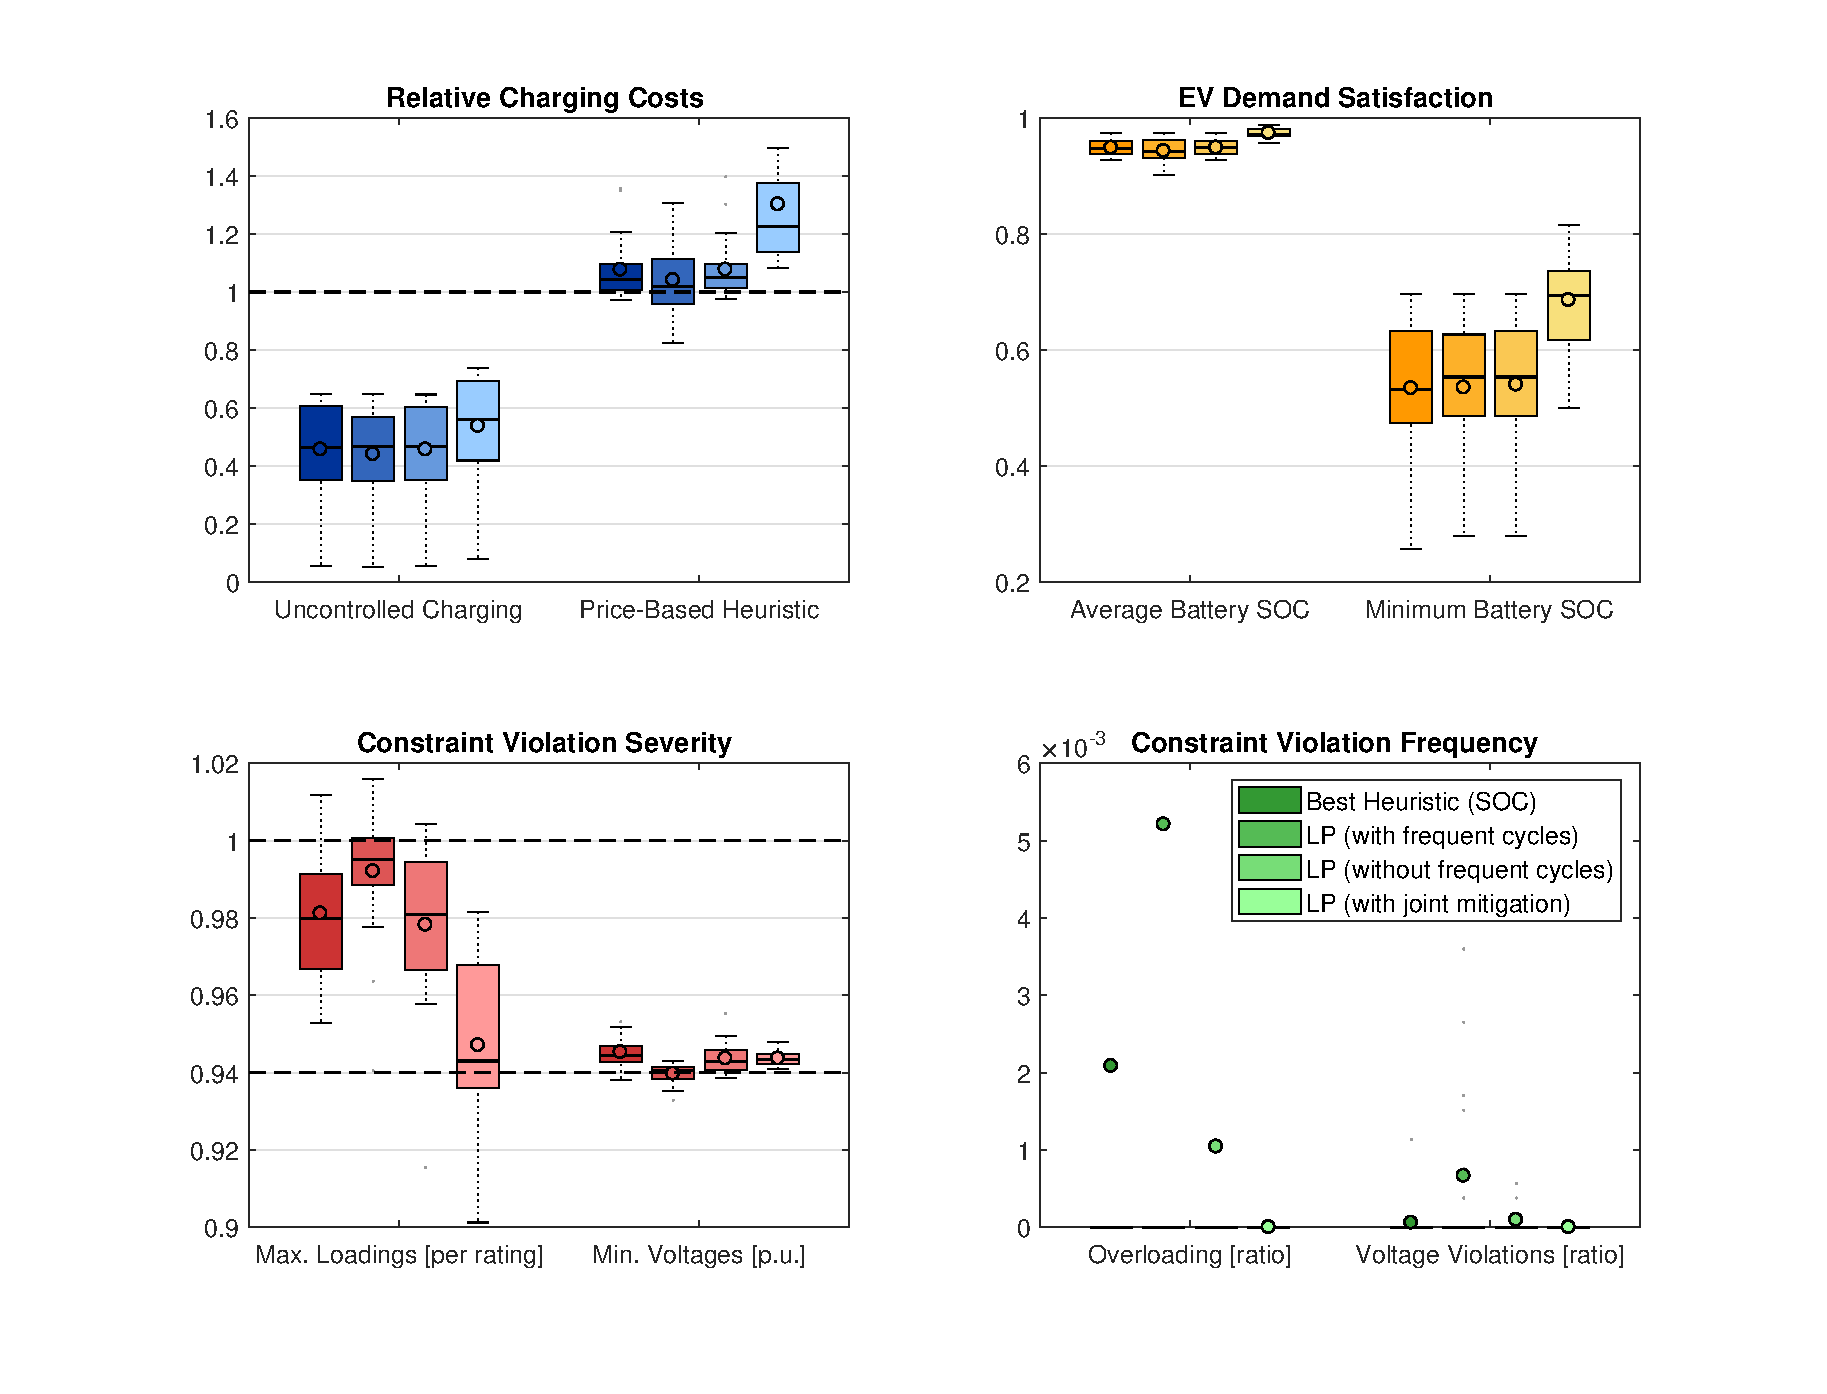
\includegraphics[width=0.98\textwidth,trim={2.9cm 1.7cm 2.5cm 0.9cm},clip]{figures/evaluation/joint.eps}
	\caption{Performance benchmark of joint uncertainty mitigation with linear programming}
	\label{fig:joint}
\end{figure}

%\vspace{-18pt}
\section{Scenario-Level Evaluation}
\label{sec:sceneval}

So far focus was put on the overall performance of different scheduling approaches across scenarios. This section is dedicated to an exemplary scenario for an in-depth study of the lost potential due to the presence of uncertainty and how schedules differ when uncertainty mitigation is applied. Therefore, \Autoref{fig:99} overlays the reference case analysis of \Autoref{fig:dumbprice} with LP results without uncertainty mitigation, with uncertainty mitigation, and ultimately an LP given perfect information about its input parameters.

\begin{figure}[]
	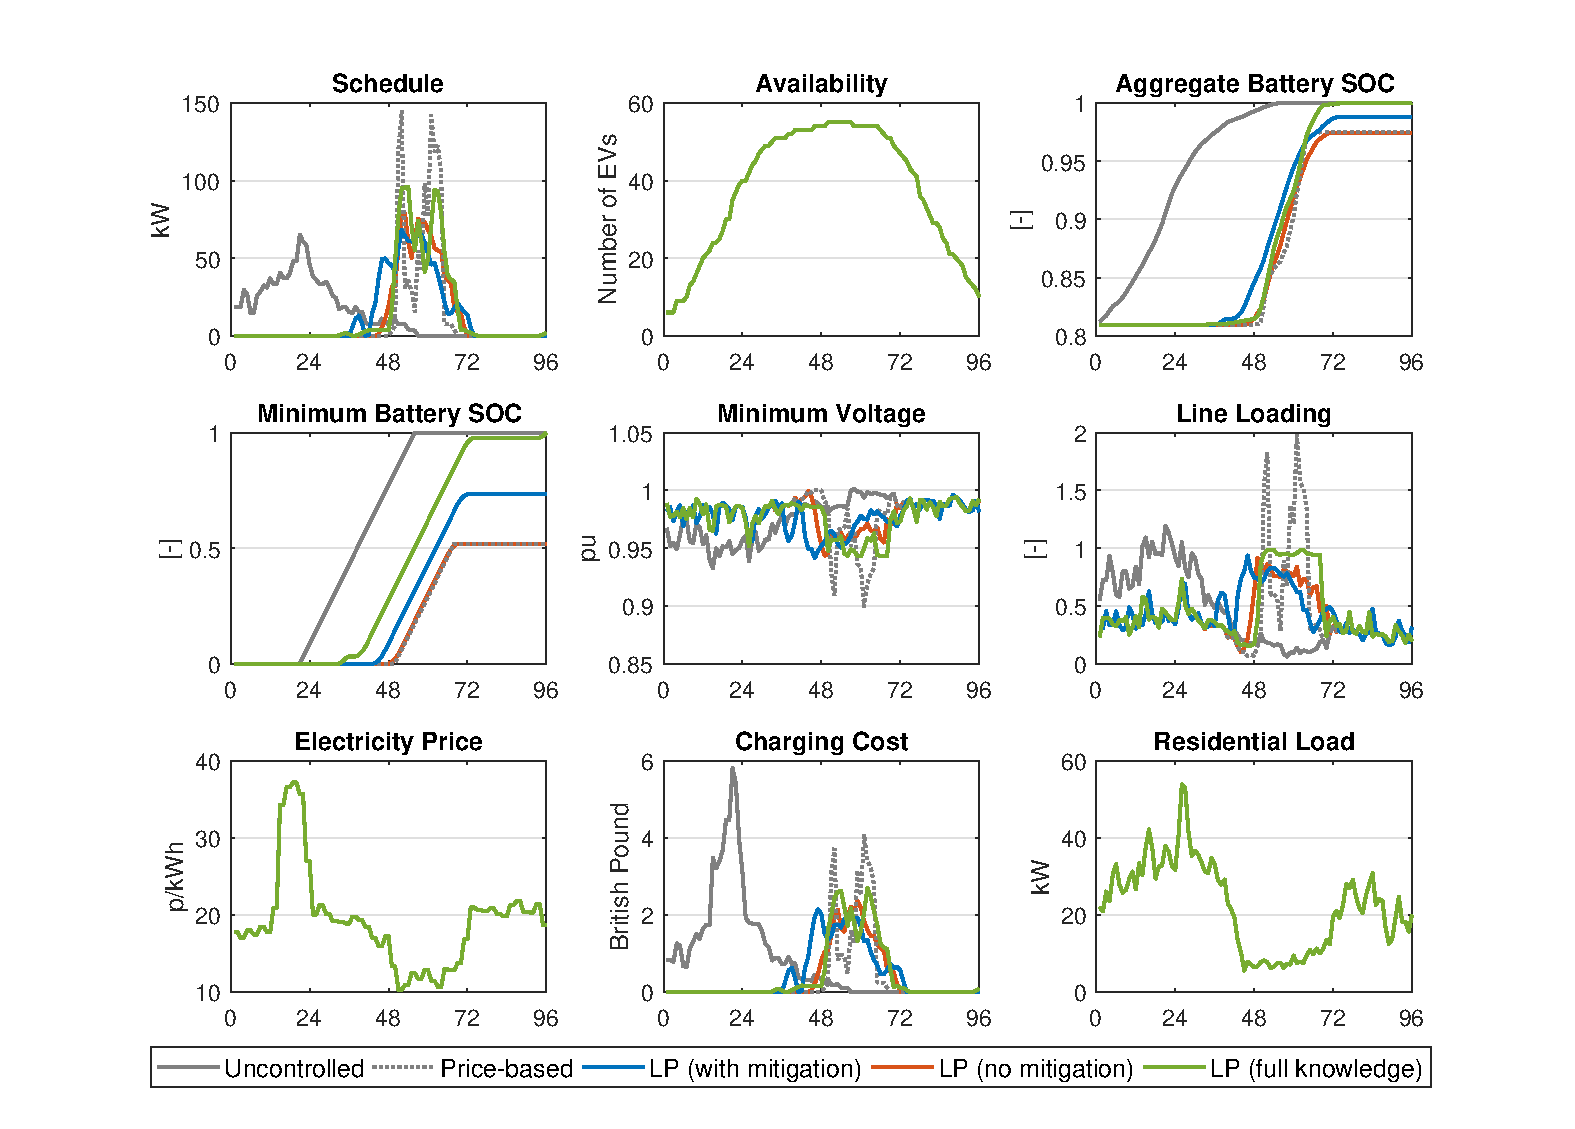
\includegraphics[width=\textwidth,trim={2cm 0cm 1.5cm 0cm},clip]{figures/evaluation/scen/99.eps}
	\caption{Comparison of linear programming with/without uncertainty mitigation}
	\label{fig:99}
\end{figure}

Clearly, loads tend to be allocated in slots with low electricity prices and high chances of availability. Moreover, they concentrate on periods of low residential demand limiting the impact of demand uncertainty and allowing substantial EV loads to be allotted in these slots. By comparison also in this specific scenario demand satisfaction is improved by uncertainty mitigation. This is achieved by increasing the scheduled energy for all EVs. Because the simple controller starts with the earliest scheduled slots and cuts off once the battery is fully charged, the resulting aggregate charge curve is shifted to earlier time slots and some of the cheapest slots are less exploited.

\begin{figure}[]
	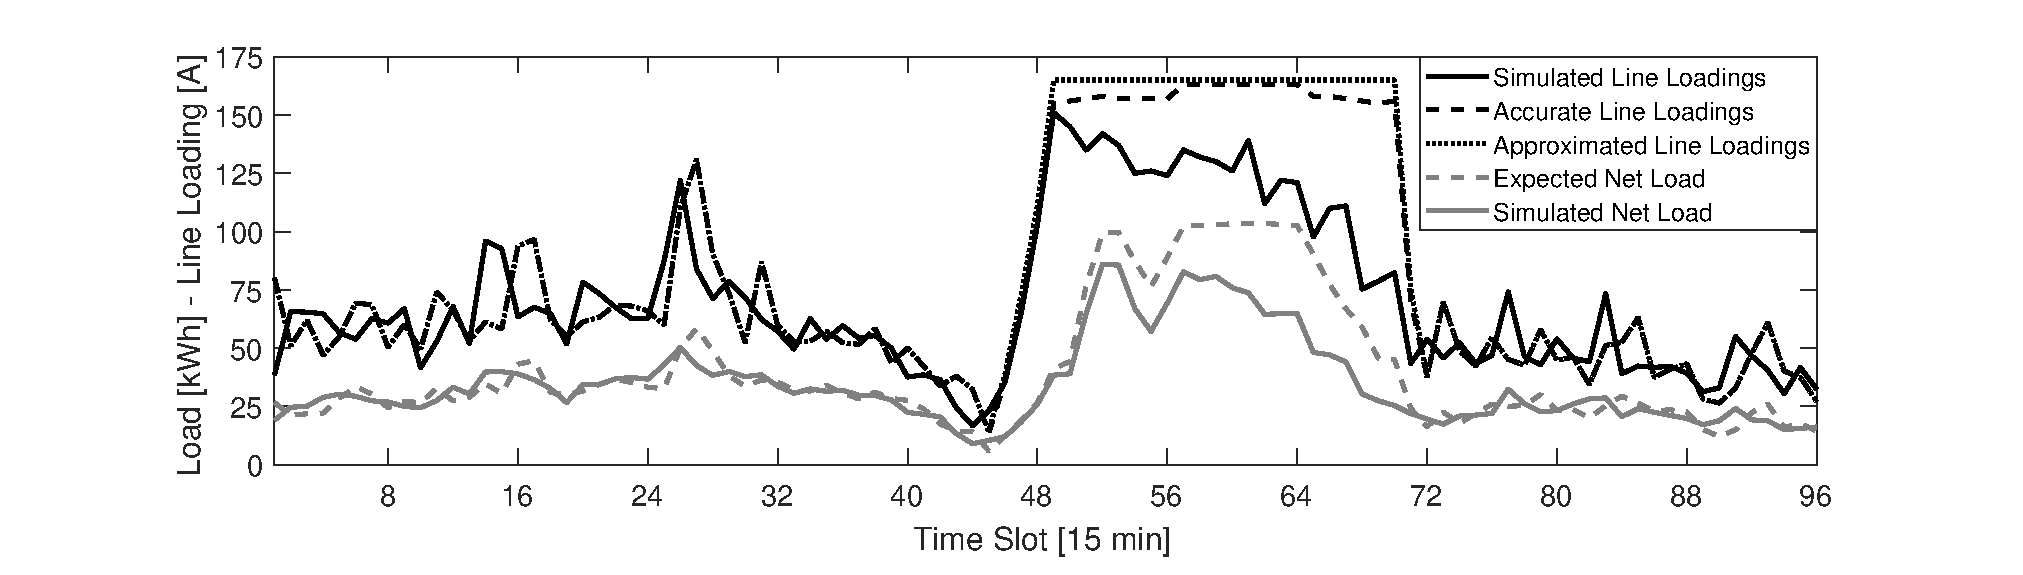
\includegraphics[width=\textwidth,trim={2cm 0.0cm 1.5cm 0cm},clip]{figures/evaluation/scen/constraints.eps}
	\caption{Constraint observation and reasons for the lack of capacity utilisation}
	\label{fig:constraints}
\end{figure}

Moreover, both LP variants lack a full capacity exploitation, the cause of which is presented in \Autoref{fig:constraints}. Approximated line loadings only play a minor role in underestimating the actual line loadings. Much more it is the net load falling short of expectations leading to a limited loading of the mains cable in inexpensive slots. A look at the LP run with perfect information supports that high rates of capacity exploitation are possible and deviations are due to prediction errors. It could further be noted that both voltage constraints, as well as maximum line loadings, take turns at causing a limitation of charging powers in respective slots.

\subsubsection*{Variation of optimal schedules due to uncertainty mitigation}

While the change in aggregate EV loads due to uncertainty mitigation was discernible from \Autoref{fig:99}, it is of further interest to examine how the schedules vary on a disaggregated level as depicted in \Autoref{fig:schedule_comparison}. First, the total charging demand increased through the lower assumed initial battery charge levels. This leads to some loads diverging from the cheapest slots. Interestingly, loads at the end of the feeder spread out more for the network is more sensitive to loads at these households. Demand uncertainty mitigation is particularly important for new charging times as they coincide more with times when residents are active. Due to its subtlety diversion from uncertain inexpensive slots cannot be observed. Further minor conceivable changes may occur through a simple exchange of charging times and rates.

\begin{figure}[]
	\centering
	\subfloat[Schedule without uncertainty mitigation]{
		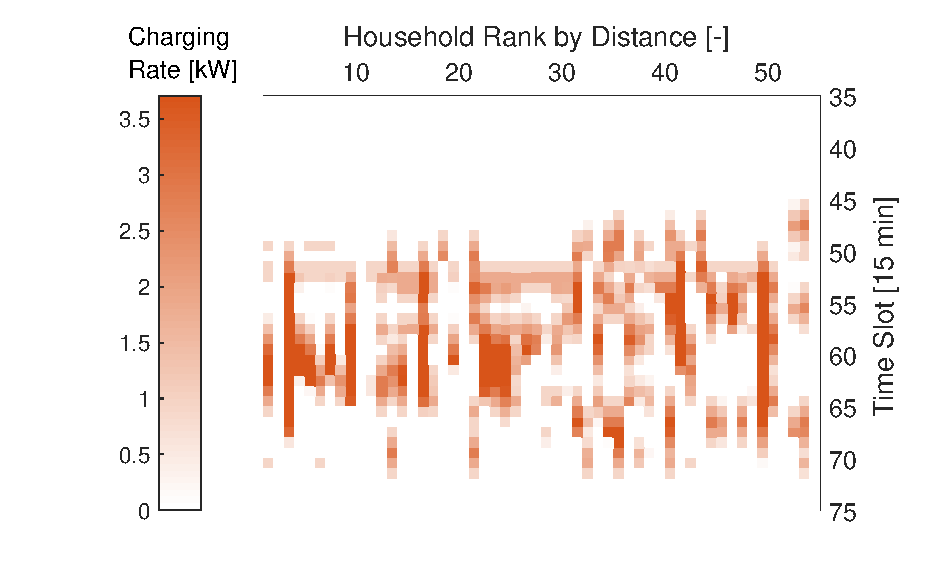
\includegraphics[width=0.48\textwidth,trim={0.2cm 0cm 0.2cm 0cm},clip]{figures/evaluation/scen/sched_nomit.eps}
		\label{fig:schednomit}
	}
	\hfill
	\subfloat[Schedule with uncertainty mitigation]{
		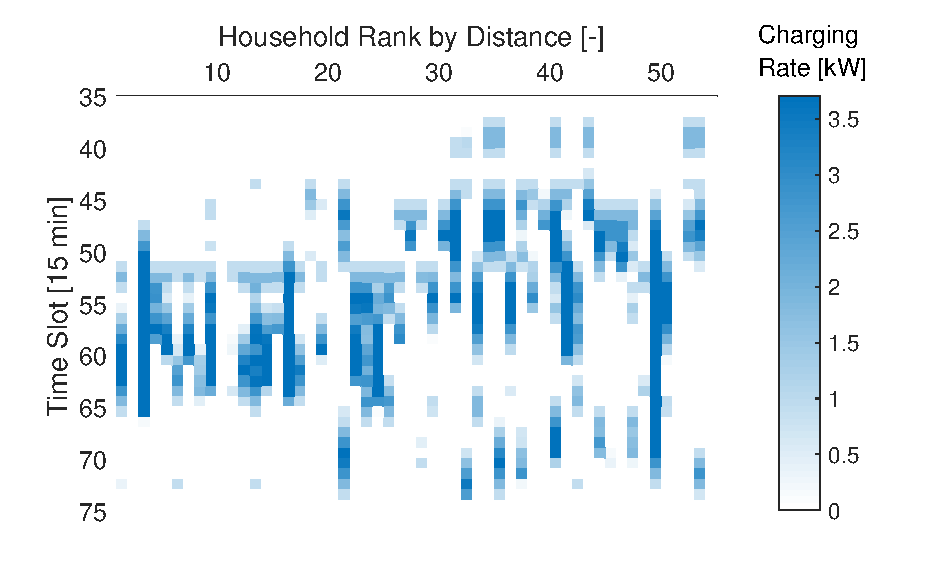
\includegraphics[width=0.48\textwidth,trim={0.2cm 0cm 0.2cm 0cm},clip]{figures/evaluation/scen/sched_mit.eps}
		\label{fig:schedmit}
	}
	\hfill
	\subfloat[Differences in schedules with and without uncertainty mitigation]{
		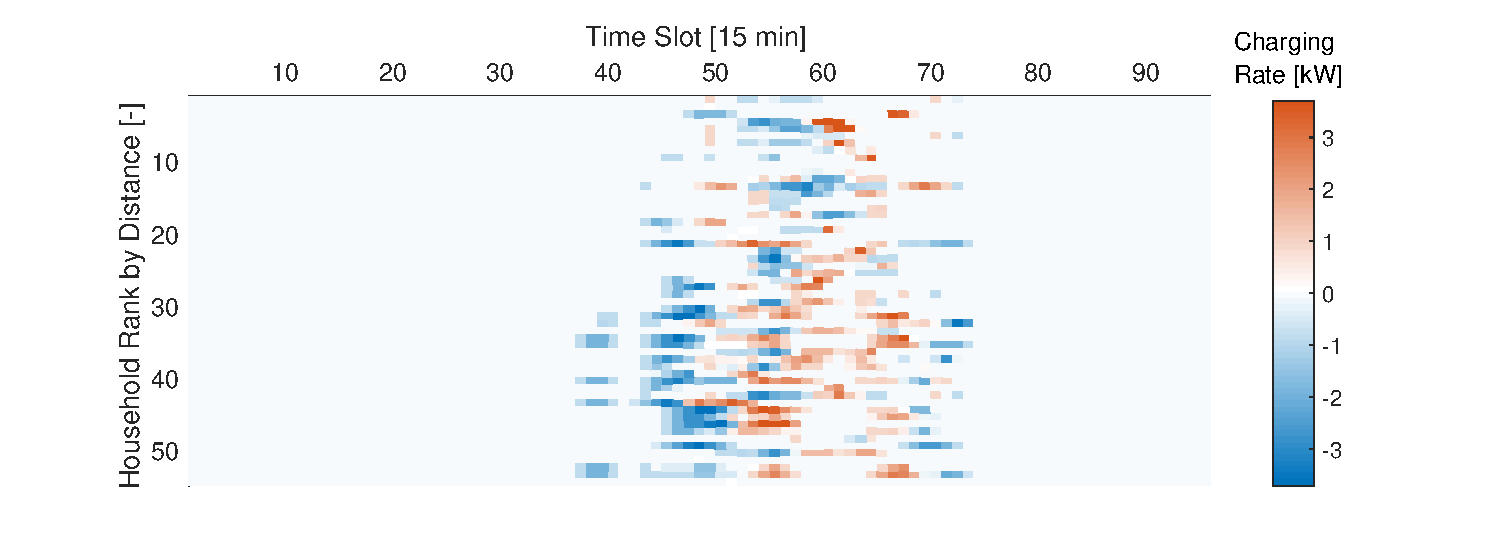
\includegraphics[width=0.95\textwidth,trim={1.5cm 0cm 2cm 0cm},clip]{figures/evaluation/scen/sched_comp.eps}
		\label{fig:schedcomp}
	}
	\caption{Optimal schedule variation due to uncertainty mitigation}
	\label{fig:schedule_comparison}
\end{figure}

\subsubsection*{Further technical issues: load losses and phase balance}

Phase imbalances have been reported to intensify in three-phase low-voltage distribution networks in the presence of electric vehicles \cite{Ul-Haq2015}. Networks are designed for loads balanced across the three phases, where currents in each phase and voltages are approximately equal. Imbalances may result in currents within the neutral line, which tends not to be rated for such currents and may lead to excessive heating \cite{Bass2013a}. This results in an increased risk of failures increases energy losses and may cause significant degradation of power quality \cite{Sun2015} as load imbalances likely entail voltage unbalances, which are in turn problematic for three-phase loads. Indeed, \Autoref{fig:phasebalance} reveals more uneven strains of individual phases for coordinated charging than for uncontrolled charging. In extreme cases, one phase is loaded less than 10 percent while others dominate with a share of more than 60 percent. Multiple means to avoid phase imbalances exist, one of which is to incorporate a phase balance constraint into the EV scheduling problem \cite{Putrus2009,Sun2015}. % FUTURE WORK

\begin{figure}[]
	\centering
	\subfloat[Uncontrolled Charging]{
		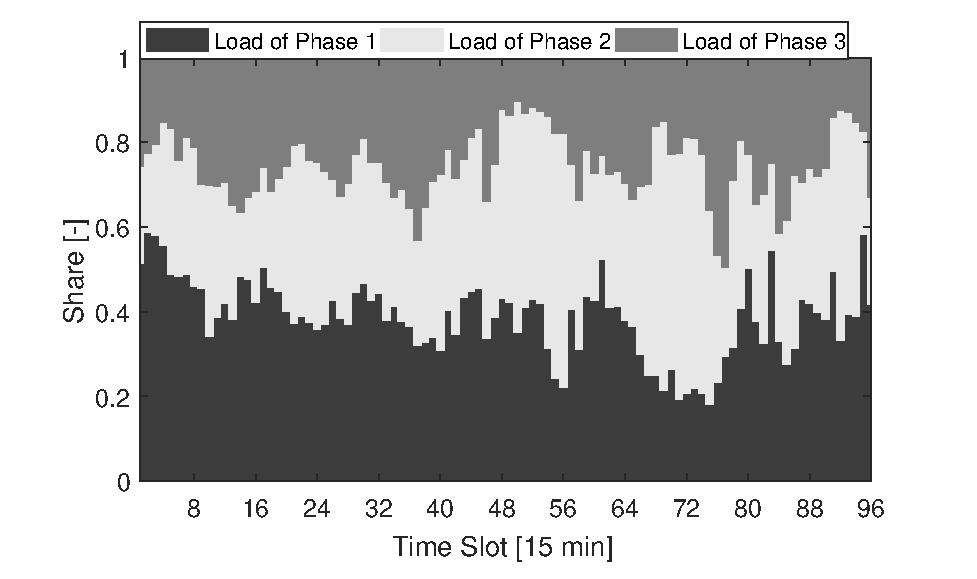
\includegraphics[width=0.48\textwidth,trim={1cm 0cm 1cm 0cm},clip]{figures/evaluation/scen/phasebalance_uc.eps}
		\label{fig:pb_uc}
	}
	\hfill
	\subfloat[LP (with uncertainty mitigation)]{
		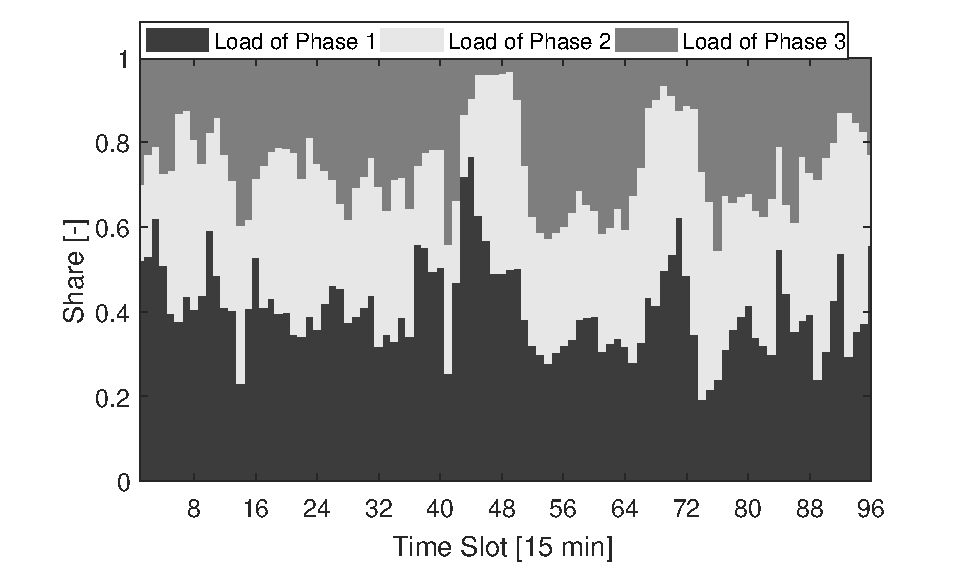
\includegraphics[width=0.48\textwidth,trim={1cm 0cm 1cm 0cm},clip]{figures/evaluation/scen/phasebalance_lp.eps}
		\label{fig:pb_lp}
	}
	\caption{Phase balance of net loads over time}
	\label{fig:phasebalance}
\end{figure}

Another concern is increased losses induced by EV scheduling. \Autoref{fig:loss} depicts load losses following the aggregate residential electricity demand including EVs. The charging rates both affect active and reactive power losses. Noteworthily, while maintaining losses in the range of less than 1\% of the total net load, the LP with uncertainty mitigation leads to an 8\% increase in losses. Hence similar to phase imbalances, the minimisation of losses may be a suitable additional objective for EV scheduling. In fact, loss minimisation has successfully been considered with regards to the limitation of EV impact on power system performance \cite{Sortomme2011, Clement2010,Deilami2011, Fazelpour2014}. However, the studies are confined to the technical optimisation and do not relate the economic benefit to the cost savings which could be obtained from price-based charging.

\begin{figure}[]
	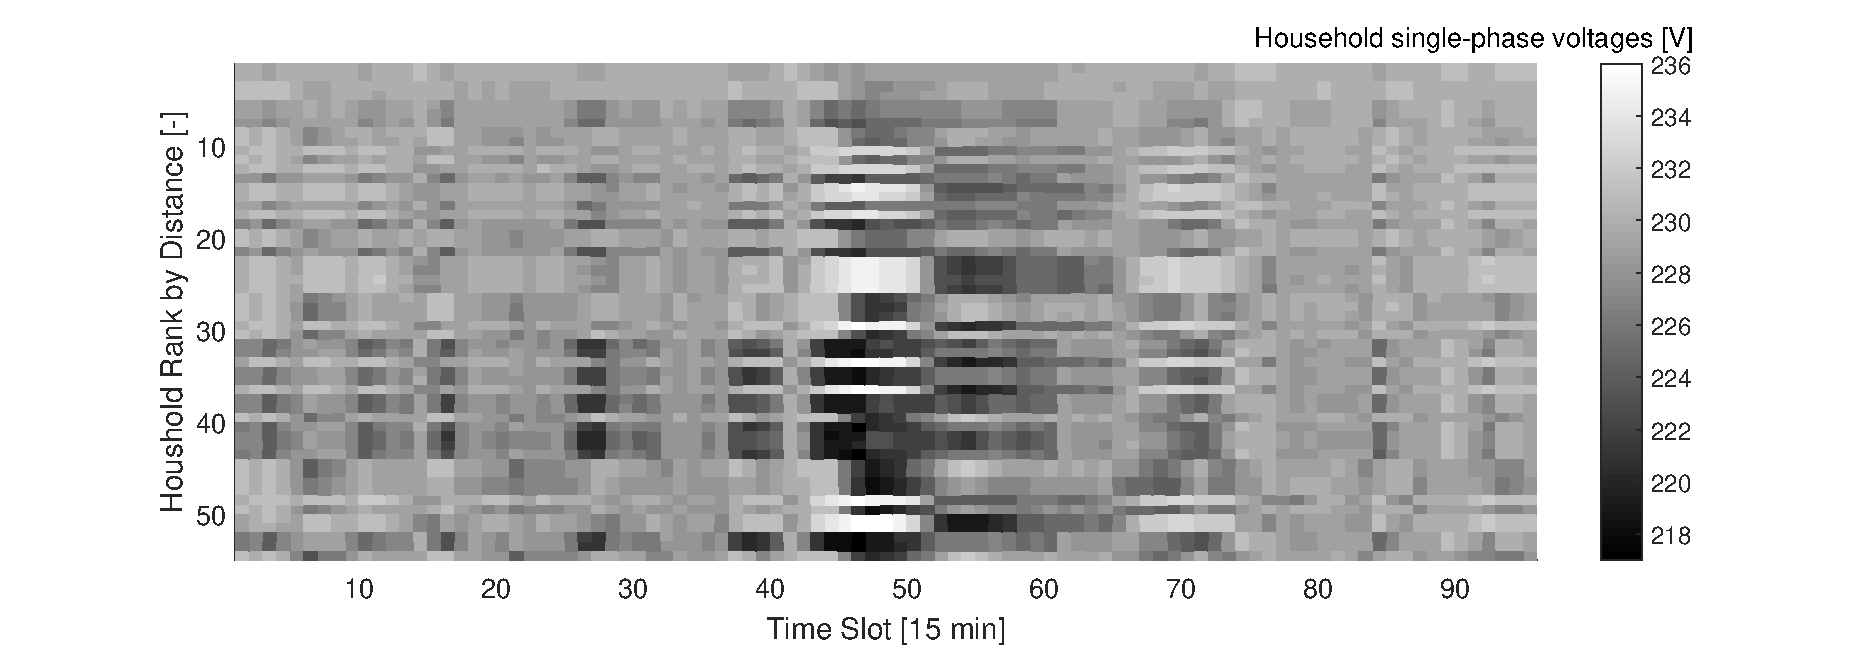
\includegraphics[width=\textwidth,trim={2cm 0cm 2cm 0cm},clip]{figures/evaluation/scen/volts.eps}
	\label{fig:volts}
	\caption{Household voltage temporal and spatial distributions (LP with uncertainty mitigation)}
\end{figure}

\begin{figure}[]
	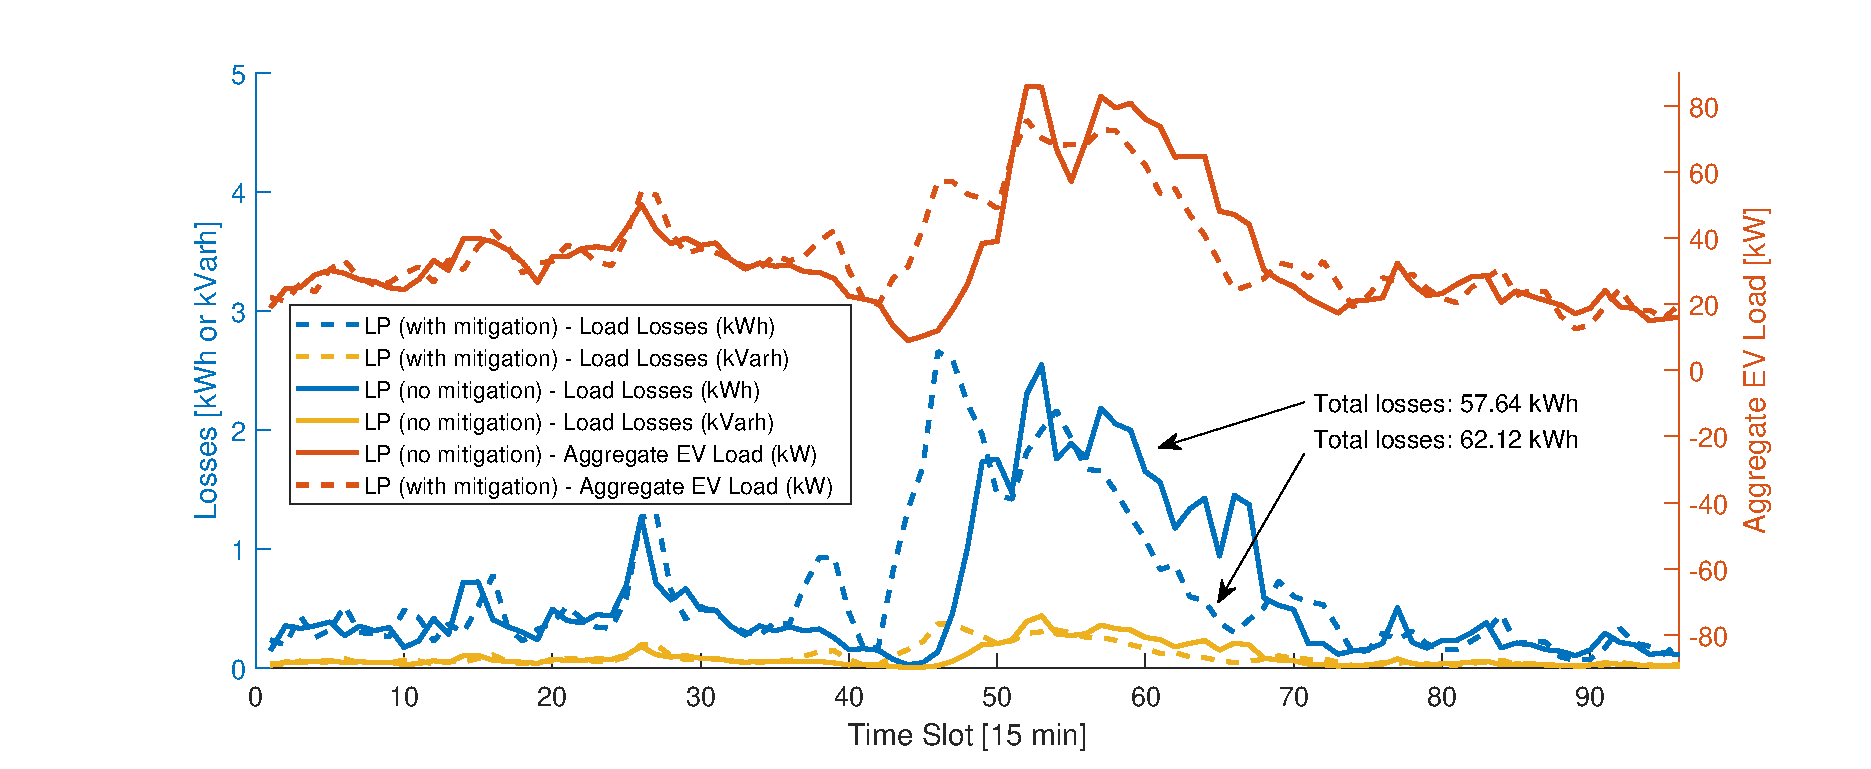
\includegraphics[width=\textwidth,trim={2cm 0cm 2cm 0.7cm},clip]{figures/evaluation/scen/losses.eps}
	\caption{Load losses in relation to aggregate EV loads}
	\label{fig:loss}
\end{figure}

\subsubsection*{Intra-scenario parameter and performance measure distributions}

Looking at the scenario parameters and selected evaluation criteria from a different angle as displayed in \Autoref{fig:hists} provides a more detailed insight into the spread achieved costs and demand satisfaction levels.

First, electricity prices range between \mbox{10-40 p/kWh} and a significant portion of prices remains below \mbox{22 p/kWh}. Because uncontrolled charging does not react to prices, average costs per household are broadly spread under the premise that consumers pay adapted wholesale prices rather than single-rate tariffs. Individual arrival times and the amount of required charge are the exclusive determinants. In comparison to the distribution of electricity prices, the histogram underlines that charging concentrates on peak demand periods with high electricity prices. Inversely, the LP without uncertainty mitigation succeeds at focussing EV loads on inexpensive and draws energy for predominantly less than \mbox{13 p/kWh} and no more than \mbox{19 p/kWh}. Thus, the cost range within which EVs are charged is small. Loads can be allocated in slots of similar prices. This changes when security constraints are applied since it causes a more even distribution of costs ranging between 10 and \mbox{19 p/kWh}. Consequently, the cost of charging is higher for some households than for others, which raises concerns about the redistribution of charging costs by the aggregator.

Second, the distributions of availability periods show that a vast majority of households are available for charging more than 12 hours per day. Coupled with the high initial battery charge levels, where a majority did not use more than 20\% of the stored energy, this exposes the high degree of flexibility of EV loads.

Third, despite the high level of freedom, not all EVs will recharge completely due to prediction errors. For both LP variants, only individual EVs could not be supplied with demanded energy due to heavy deviations from behaviour predictions, i.e.\ vehicles were available only for an insufficient time or had a shallow initial battery charge level. However, the LP with uncertainty mitigation could lift final battery charge levels from the interval $[0.9,0.95]$ to the next $[0.95,1.0]$ affecting around 10\% of vehicles.

\begin{figure}[]
	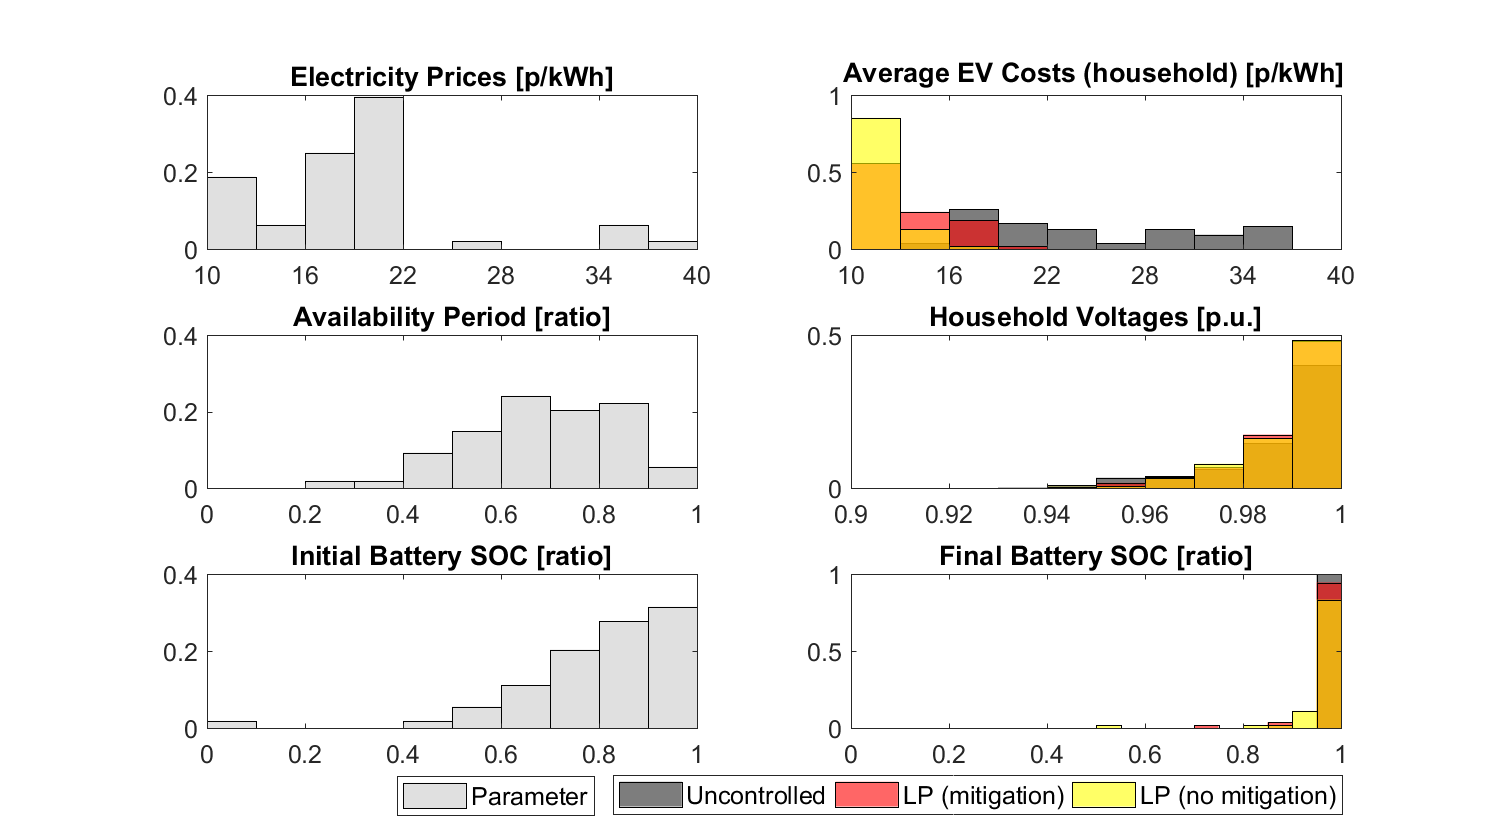
\includegraphics[width=0.9\textwidth,trim={1cm 0cm 1cm 0.5cm},clip]{figures/evaluation/scen/hists.eps}
	\caption{Histograms of scenario parameters and selected evaluation criteria}
	\label{fig:hists}
\end{figure}

\section{Household-Level Evaluation}
\label{sec:hdeval}

To complement the scenario-level evaluation, two exemplary households were picked to gain insight into the implication of EV scheduling to individual households with regards to their point of connection, the uncertainty involved and functioning principle of the controller. 

\begin{figure}[]
	\centering
	\subfloat[Household 17 (close to substation)]{
		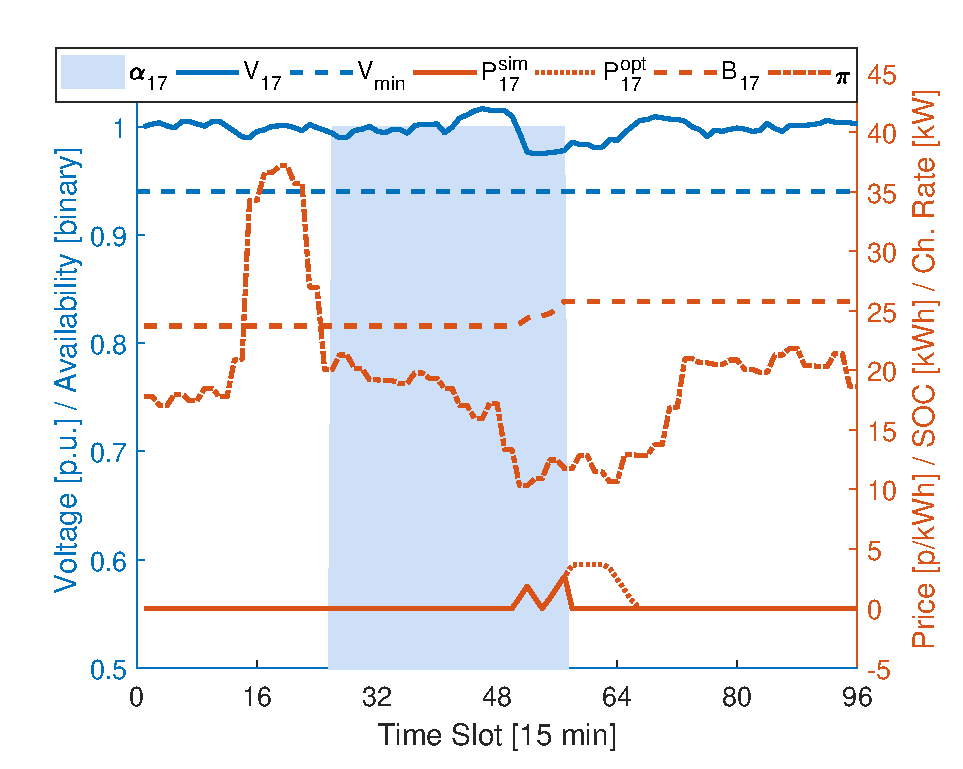
\includegraphics[width=0.48\textwidth]{figures/evaluation/ind/ind17.eps}
		\label{fig:ind17}
	}
	\hfill
	\subfloat[Household 54 (far from substation)]{
		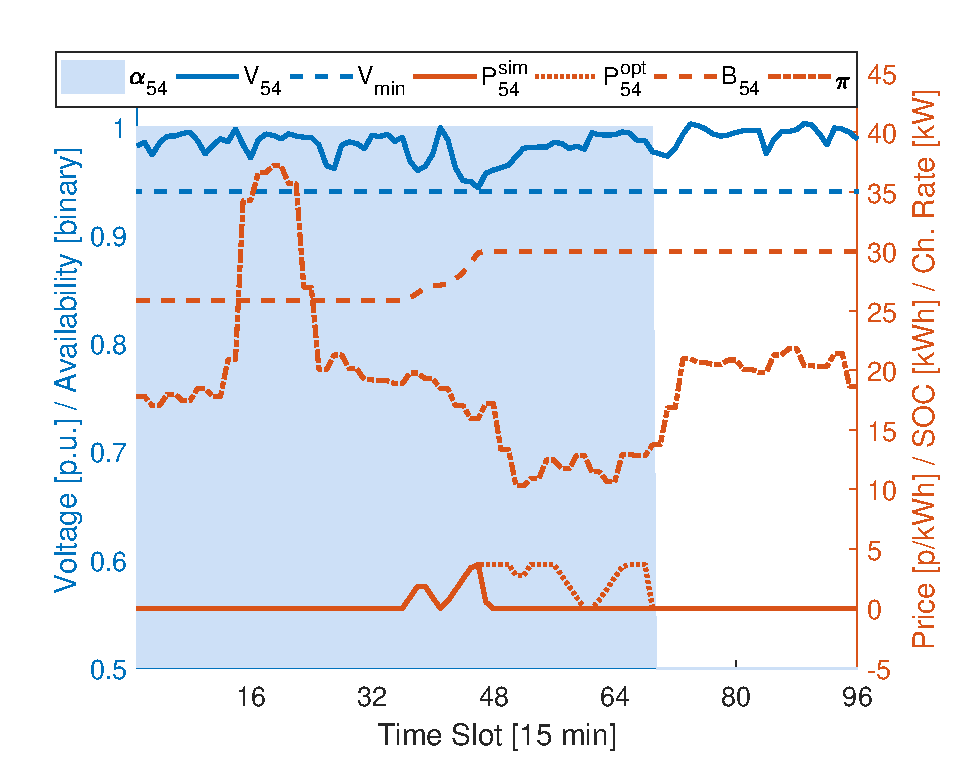
\includegraphics[width=0.48\textwidth]{figures/evaluation/ind/ind54.eps}
		\label{fig:ind54}
	}
	\caption{Household-level effect of point of connection, uncertainty, and controller}
	\label{fig:examplehds}
\end{figure}

\Autoref{fig:ind17} shows the characteristics of a home close to the substation. It generally exhibits high bus voltages, which are weakest when EV charges locally. Overall, voltages tend to weaken when the price is low, and EV loads are allocated elsewhere. Periods, where the electric vehicle is available, are shaded. It becomes apparent that the day-ahead schedule failed to predict the availability period correctly. Due to low prices, the vehicle was scheduled to charge in a period where availability was predicted. However, because the vehicle departed earlier than expected and planned charging processes are missed, the battery could not be refilled completely.

Conversely, \Autoref{fig:ind54} shows the features of a household located further away from the transformer. Lower voltages persist throughout the optimisation horizon, but similarly, voltages are weakest when the corresponding vehicle is charged, and lower voltages coincide either with peak residential demand or EV loads elsewhere prompted by low electricity prices. Furthermore, it exhibits another peculiarity related to the battery state of charge uncertainty mitigation. Because the initial battery charge level is higher than expected, the battery is fully charged before the schedule is exhausted. The controller prevents the battery from overcharging, but it is easily discernible that the loads reserved for this household and expected to strain cables and deteriorate voltages could have been allocated to another EV whose load ipso facto could not be accommodated.

\section{Sensitivity of Cost Saving Potential Towards Price Variance}
\label{sec:pseval}

The prospect of real-time electricity prices (RTP) has caused worries for both customers and utilities. While customers fear an increase in average retail prices, utilities are afraid of a revenue shortfall. In fact, RTP promise lower costs through reduced peak loads and increased reliability via a reduced likelihood of system shortages and blackouts \cite{Borenstein2002}. Generally, customers with a flatter demand profile will benefit more than customers with rather peaky consumption patterns and customers with numerous deferrable loads will realise larger cost reductions than static customers \cite{Borenstein2002}. However, the extent of cost savings will ultimately not only depend on the customer's flexibility but also on the variance of electricity prices.

\begin{figure}[]
	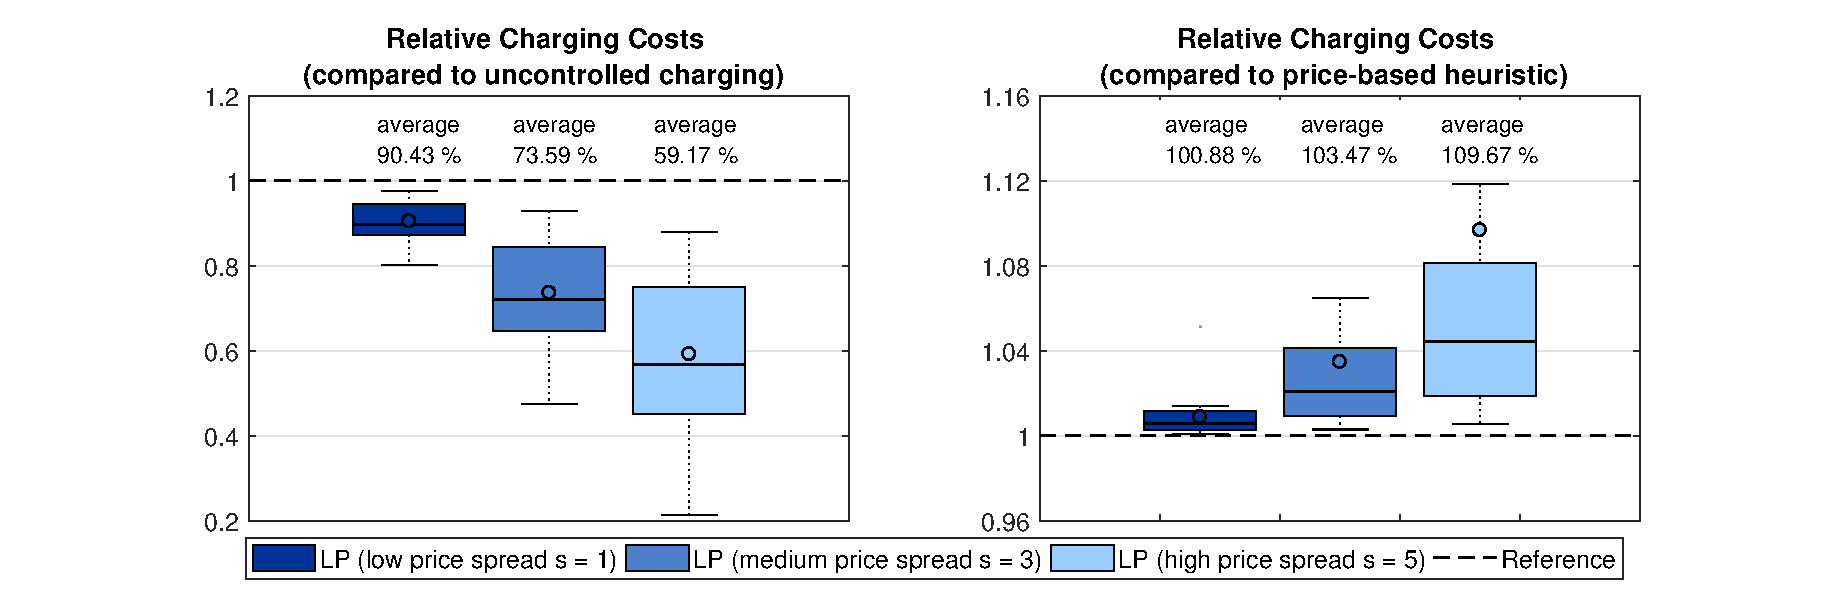
\includegraphics[width=\textwidth,trim={3cm 0cm 2.5cm 0cm},clip]{figures/evaluation/spreads.eps}
	\caption{Sensitivity of relative charging costs to different price spreads}
	\label{fig:spreads}
\end{figure}

This influence is analysed by running the presented EV scheduling method for each low, medium, and high spreading factors. It is shown that the more price signals were spread, the more savings could be achieved compared to uncontrolled charging. According to \Autoref{fig:spreads}, average charging cost reductions decrease linearly from 10\% via 26\% to 41\%. However, naturally, the range of cost savings increases reducing the certainty about the daily revenue. This, however, is a second-tier issue as the aggregator reports on a long-term basis. Most strikingly, it highlights that the cost saving potential is insufficient for today's market and electricity retail structure with dominating static surcharges. If, for instance, the average annual electricity demand of an electric vehicle is 4,000 kWh and the current average single-rate tariff is \mbox{17 p/kWh} the charging cost would amount to \pounds 680.00. A reduction to 90\% of this value would result in absolute annual cost savings of \pounds 68.00. This small potential is unlikely to trigger vehicle owners to devise charging control to a central aggregator, let alone offer an economic foundation for aggregators to flourish \cite{Bessa2010}. The increase by a fourfold, however, may change this perception; an outlook on savings of \pounds 272.00 sounds more intriguing against the backdrop of total anticipated charging costs of \pounds 680.00.

The analysis underlines that the integration of EV load flexibilities into the market requires dependable financial incentives to cover investment costs in charging, control, and vehicle infrastructure. As pointed out earlier, wholesale market prices for end-users are burdened with a variety of additive levies, charges, and taxes, which reduce the price signals in their relevance and make them unattractive for demand side management. To unfold the incentive effect of market prices, it is proposed to redesign surcharges by dynamising these additive price components. Instead of charging the same amount of levy for each unit of electricity consumed, the corresponding price component is adjusted employing a market indicator such as the spot price. If the price is low, only a small surcharge is due. When spot prices are high, the shortage signal reflecting the overall network state is amplified.

This incentive proposition is advantageous as it does not influence the price-setting mechanism on the electricity market since the surcharges only affect consumers. Besides, a regional adjustment is possible, depending on the design, to not only reflect bottlenecks in the transmission system but also on distribution networks. Instead of a static subsidy with significant fiscal implications, owners are affirmatively nudged to exploit available renewable power generation through the amplification of the price signal. Most intriguingly, it may be fiscally neutral if efficiently implemented and anticipated systematic load shifts to cheaper periods are priced in. The major drawbacks are high expected administrative, and operative efforts end the concern that adaptations under changing market conditions reduce the planning security of consumers and, predominantly, aggregators.

Besides the experiment showed that through increased price spreads the relative costs of shifting loads away from the cheapest time slots to observe technical constraints inherently increases. Alternative slots are relatively more expensive. While for today's price spreads the average cost increase is confined to 1\%, lost profits ascend to almost 10\% for spreading factor 5 including numerous outliers.
